\documentclass[12pt]{report}

\usepackage[T1]{fontenc}
\usepackage[italian]{babel}
\usepackage[hidelinks]{hyperref}
\usepackage{tikz, pgfplots}
\usepackage{graphicx}
\usepackage{tabularx}

\hypersetup {
    colorlinks=true,
    urlcolor=blue,
    linkcolor=blue
}

% --------------- STYLE ---------------
\usepackage[margin=1.25in]{geometry}
\usepackage{xcolor}

\usepackage{fancyhdr}
\usepackage[Sonny]{fncychap}
\usepackage[most]{tcolorbox}

% Font
\renewcommand{\familydefault}{\sfdefault}
\usepackage{sansmath}
\sansmath

\pagestyle{fancy}
\setlength{\headheight}{15pt}
\rhead{\thepage}


% --------------- MATH ---------------
\usepackage{amsmath, amssymb, amsthm, amsfonts, mathtools}

\usepackage{mdframed}
\newtheoremstyle{th_style}
{0pt}{0pt}
{\normalfont}
{}
{\color{green!40!black}}
{\;}{0.25em}
{\thmname{\textbf{#1}}\thmnumber{ \textbf{#2}}{\color{black}\thmnote{\textbf{ -- #3}}}}

\newmdenv[
	rightline=false,
	leftline=true,
	topline=false,
	bottomline=false,
	linecolor=green!40!black,
	innerleftmargin=5pt,
	innerrightmargin=5pt,
	innertopmargin=5pt,
	innerbottommargin=5pt,
	leftmargin=0cm,
	rightmargin=0cm,
	linewidth=4pt
]{dBox}

\newmdenv[
	rightline=false,
	leftline=true,
	topline=false,
	bottomline=false,
	linecolor=green!40!black,
	backgroundcolor=black!5,
	innerleftmargin=5pt,
	innerrightmargin=5pt,
	innertopmargin=5pt,
	innerbottommargin=5pt,
	leftmargin=0cm,
	rightmargin=0cm,
	linewidth=4pt
]{pBox}

\theoremstyle{th_style}
\newtheorem{theoremeT}{Teorema}[chapter]
\newtheorem{definitionT}{Definizione}[chapter]
\newtheorem{propositionT}{Proposizione}[chapter]
\newtheorem{corollary}{Corollario}[chapter]
\newtheorem{lemma}{Lemma}[chapter]
\newtheorem{observation}{Osservazione}[chapter]
\newtheorem{exampleT}{Esempio}[section]

\newenvironment{theorem}{\begin{pBox}\begin{theoremeT}}{\end{theoremeT}\end{pBox}}
\newenvironment{definition}{\begin{dBox}\begin{definitionT}}{\end{definitionT}\end{dBox}}
\newenvironment{proposition}{\begin{pBox}\begin{propositionT}}{\end{propositionT}\end{pBox}}
\newenvironment{example}{\begin{dBox}\begin{exampleT}}{\end{exampleT}\end{dBox}}


\pgfplotsset{compat=newest}

\newcommand{\N}{\mathbb{N}}
\newcommand{\Z}{\mathbb{Z}}
\newcommand{\R}{\mathbb{R}}
\newcommand{\RR}{\mathcal{R}}
\newcommand{\C}{\mathcal{C}}
\newcommand{\F}{\mathbb{F}}
\newcommand{\K}{\mathcal{K}}
\newcommand{\B}{\mathcal{B}}
\renewcommand{\P}{\mathcal{P}}
\newcommand{\NP}{\mathcal{NP}}
\renewcommand{\O}{\mathcal{O}}

\newcommand{\tx}{\tilde{x}}
\newcommand{\norm}[1]{\left\lVert#1\right\rVert}
\newcommand{\start}{\triangleright}

\DeclareMathOperator{\sign}{sign}
\DeclareMathOperator{\trn}{trn}
\DeclareMathOperator{\arr}{arr}
\DeclareMathOperator{\fl}{fl}
\DeclareMathOperator{\dist}{dist}
\DeclareMathOperator{\Ker}{Ker}
\DeclareMathOperator{\diag}{diag}
\DeclareMathOperator{\nnz}{nnz}
\DeclareMathOperator{\Var}{Var}
\DeclareMathOperator{\LS}{LOGSPACE}
\DeclareMathOperator{\TIME}{TIME}

\title{Elementi di calcolabilità e complessità}
\author{Federico Bustaffa}
\date{15/04/2024}

\begin{document}

\maketitle

\begin{abstract}
	Lo scopo di questi appunti è rendere la comprensione dei
	concetti spiegati all'interno del corso il più semplice
	possibile fornendo esempi e spiegazioni quasi ad un livello
	divulgativo per quanto mi sia possibile.

	Non mancheranno il rigore e i formalismi spiegati a lezione
	una volta definite le basi per poterli comprendere.

	Ovviamente questi appunti rispecchiano la mia personale
	interpretazione dei concetti mostrati all'interno del corso
	e dunque anche i miei limiti di apprendimento degli stessi.

	Il corso sarà suddiviso in due parti: la prima tratterà la
	teoria della \textbf{calcolabilità}, mentre la seconda la
	teoria della \textbf{complessità}.
\end{abstract}

\tableofcontents

% -------------- CALCOLABILITA' -------------------
\part{Ricerca}
\chapter{Introduzione}
L'intelligenza artificiale si occupa della comprensione e riproduzione del
comportamento \emph{intelligente}. Nello specifico, l'intelligenza pu\`o riguardare
le sole facolt\`a mentali, ovvero il ragionamento, oppure l'azione umana in senso
pi\`u ampio, ovvero il comportamento.

\section{I diversi approcci all'IA}
\subsection{Approccio psicologico cognitivo}
Da un lato vediamo l'IA come una scienza che si basa sulla sperimentazione e possiamo
definire questo approccio come \textbf{approccio della psicologia cognitiva}.

Qui  l'obbiettivo \`e quello di comprendere l'intelligenza umana e costruire dei
modelli computazionali che sono poi sottoposti ad una verifica sperimentale.

Il criterio di successo \`e capire i meccanismi che stanno alla base
dell'intelligenza umana per poi risolvere i problemi con gli stessi processi usati
dall'uomo.

\subsection{Approccio costruttivo}
Dall'altro possiamo vedere l'IA come una disciplina informatica in cui si cerca di
costruire entit\`a dotate di intelligenza senza perforza essere legati al modello di
intelligenza umana.

L'obbiettivo \`e quello codificare quelli che sono il pensiero e il comportamento
\emph{razionale} cos\`i come li conosciamo.

Il criterio di successo \`e risolvere problemi che richiedono intelligenza, non
importa come.

\subsection{Una definizione di IA}
Possiamo riassumere ci\`o che abbiamo detto prima con la seguente definizione di
intelligenza artificiale: Il settore dell'IA consiste nell'indagine tecnologica e
intellettuale che mira al raggiungimento dei seguente obbiettivi:
\begin{itemize}
	\item Costruzione di macchine intelligenti, sia che operino come l'uomo che
	      diversamente.
	\item Formalizzazione della conoscenza e meccanizzazione del ragionamento, in
	      tutti i settori di azione dell'uomo.
	\item Comprensione mediante modelli computazionali della psicologia e
	      comportamento di uomini, animali e agenti artificiali.
	\item Rendere il lavoro con il calcolatore altrettanto facile e utile del lavoro
	      con persone capaci, collaborative e possibilmente esperte.
\end{itemize}

\section{Capacit\`a dell'IA}
Ma che tipo di capacit\`a deve avere un agente intelligente ? La definizione di
intelligenza non \`e unica e nemmeno il tipo di intelligenza lo \`e. Ecco perch\'e,
in base al tipo di agente intelligente e al problema che deve risolvere si enfatizza
un tipo di intelligenza piuttosto che un altro. Vediamo alcune delle capacit\`a che
pu\`o avere uno di questi agenti:
\begin{itemize}
	\item Simulazione del comportamento umano.
	\item Ragionamento logico/matematico.
	\item Competenza in un certo ambito.
	\item Buon senso (senso di collettivit\`a).
	\item Efficienza nell'interazione con un certo ambiente.
	\item Socialit\`a e collaborazione.
	\item Emozioni.
	\item Apprendimento.
	\item Creativit\`a.
\end{itemize}

\section{Test di Turing}
Il test di Turing consiste nel far dialogare una persona (interrogatore)
contemporaneamente con un'altra persona e con una macchina (chat bot) per cinque
minuti. Se il 30\% degli interrogatori non riesce a distinguere la persona dalla
macchina allora la macchina ha superato il test ed \`e quindi considerata
"\emph{intelligente}".

Questo test non \`e pi\`u cos\`i utilizzato per definire "\emph{intelligente}" una
macchina perch\'e non sempre l'intelligenza che vogliamo misurare \`e coerente col
test e perch\'e non sempre l'intelligenza artificiale si basa sulla simulazione.

\section{Breve storia}
Nel 1943 Mc Culloch e Pitts pubblicano il primo lavoro sulle reti neurali, nel 1949 arriva
il lavoro di Hebb. Nel 1956, durante la conferenza di Darthmouth viene coniato il termine
"\emph{Intelligenza Artificiale}".

Si raggiunge una \textbf{capacit\`a di ragionamento simbolico}, ovvero l'intelligenza riesce a
risolvere problemi utilizzando simboli di un determinato linguaggio. Per esempio \`e possibile
tradurre frasi in linguaggio naturale in proposizioni logiche che poi vengono trattate.

Si riesce anche a far giocare a scacchi una macchina che riesce a battere il campione mondiale
di scacchi. Il computer usato riusciva a valutare 200 milioni di mosse al secondo e conosceva
600.000 aperture.

In seguito a questi traguardi le aspettative erano alte: si riescono a fare programmi in grado
di dimostrare teoremi, sistemi basati su conoscenza (fornisco in anticipo delle conoscenze al
programma), vengono risolti problemi su dei cosidetti "\emph{micromondi}".

In seguito ci si rende conto che la manipolazione simbolica non \`e pi\`u adeguata a molti tipi
di problema, che la complessit\`a dei problemi va incontro ad una
\textbf{intrattabilit\`a computazionale}, che ci sono limiti alla rappresentazione delle rete
neurali di tipo semplice (\textbf{percettroni}).

Con l'arrivo dei \textbf{sistemi esperti} si riesce a risolvere tanti dei problemi a cui si era
andati incontro. Questi sistemi sono specializzati sul risolvere problemi specifici e conoscono
molto bene il dominio di questi ultimi. Questi sistemi tuttavia fallivano su problemi molto
banali poich\'e sprovveduti di \textbf{senso comune}, che comunque era qualcosa di molto
vasto e difficile da codificare.

Nel 1986 c'\`e il ritorno delle \textbf{reti neurali}, con algoritmi basati sulla
\textbf{retropropagazione} che si sostituiscono ai modelli a ragionamento simbolico,
dominanti all'epoca. Con questo ritorno si adottano sempre di pi\`u sistemi basati sul
\textbf{ragionamento probabilistico} e sull'\textbf{apprendimento automatico}.

\section{Idea intuitiva di algoritmo} \label{sec: algoritmo}
Tralasciando i molti formalismi proposti per esprimere algoritmi,
in ognuno di essi, un \textbf{algoritmo} deve soddisfare i
seguenti requisiti
\begin{enumerate}
	\item Deve essere costituito da un insieme \emph{finito} di
	      istruzioni.
	\item Le istruzioni possibili sono in numero \emph{finito}
	      e hanno effetto \emph{limitato} su dati discreti,
	      esprimibili in maniera finita.
	\item Una computazione è eseguita per \emph{passi discreti},
	      senza ricorrere a sistemi analogici o metodi continui,
	      ciascuno dei quali impiega un tempo \emph{finito}.
	\item Ogni passo dipende solo dai precedenti e da una
	      porzione finita dei dati, in modo
	      \emph{deterministico}.
	\item Non c'è limite al numero di passi necessari
	      all'esecuzione di un algoritmo, né alla memoria
	      richiesta per contenere i dati iniziali, intermedi ed
	      eventualmente finali.
\end{enumerate}
Sotto queste ipotesi, tutte le formulazioni fino ad ora
sviluppate sono equivalenti e si postula che lo saranno anche
tutte le future.



\chapter{Macchine di Turing}
Introduciamo il primo formalismo per esprimere algoritmi, ideato
da Alan Turing nel 1936 e che prende il nome di
\textbf{macchina di Turing}.

L'idea di base è quella di avere un \textbf{nastro} di lunghezza
infinita su cui disporre una stringa di caratteri, rappresentante
l'input dell'algoritmo. Tale macchina è dotata di un
\textbf{cursore} che, partendo dall'inizio della stringa, legge
i caratteri che incontra e, in base a cosa legge, cambia stato
e si muove. La computazione termina quando si giunge finalmente
in uno stato speciale di terminazione.

\begin{definition}
	Una \textbf{macchina di Turing} (MdT) è definita come una
	quadrupla di questo tipo
	\[
		M = \begin{pmatrix}
			Q, & \Sigma, & \delta, & q_0
		\end{pmatrix}
	\]
	dove
	\begin{itemize}
		\item $Q$ è l'\textbf{insieme finito degli stati} in
		      cui si può trovare la macchina. Tra gli stati
		      abbiamo uno stato speciale $h$, con cui
		      indicheremo la corretta terminazione del calcolo
		      della macchina $M$.
		\item $\Sigma = \{ \sigma, \sigma', \dots \}$ è
		      l'\textbf{insieme finito dei simboli}, ossia,
		      l'\textbf{alfabeto} utilizzato per esprimere
		      gli algoritmi. Il numero e e i simboli stessi
		      possono variare da una MdT all'altra, tuttavia
		      ci sono dei simboli considerato speciali che sono
		      sempre presenti:
		      \begin{itemize}
			      \item \textbf{Bianco}: indicato con $\#$ è
			            come un carattere nullo.
			      \item \textbf{Respingente}: indicato con
			            $\start$, simboleggia l'inizio delle
			            stringa. Il cursore della macchina non
			            può andare mai a sinistra di questo
			            simbolo.
			      \item \textbf{Spostamento}: simboli che non
			            appartengono a $\Sigma$ e indicano come
			            e in che direzione muovere il cursore.
			            Sono rispettivamnete $L$, $R$ e $-$ che
			            stanno per \verb|Left|, \verb|Right| e
			            \verb|Hold| (non muovere il cursore).
		      \end{itemize}
		\item \textbf{Stato iniziale}: indicato con $q_0 \in Q$
		      è lo stato iniziale in cui si trova la macchina.
		\item \textbf{Funzione di transizione}: indicata con
		      $\delta$ è la funzione che definisce la
		      transizione da uno stato all'altro della macchina
		      in base a quel che viene letto dal cursore e in
		      base a quel che è stato letto fino a quel momento.
		      \[
			      \delta \subseteq (Q \times \Sigma) \to
			      (Q \cup \{ h \}) \times \Sigma \times
			      \{ L, R, - \}
		      \]
		      che ci permette per l'appunto di cambiare lo
		      stato della macchina e progredire nel calcolo.
	\end{itemize}
\end{definition}

\section{Funzione di transizione}
La \textbf{funzione di transizione} $\delta$ è necessaria a
far progredire il calcolo. Come possiamo vedere dalla
definizione che ne abbiamo dato, questa prende in input una
coppia di valori.
\begin{itemize}
	\item Lo \textbf{stato corrente} $q$ della macchina.
	\item Un simbolo $\sigma$ dell'alfabeto
\end{itemize}

Notiamo inoltre che la funzione $\delta$ prende in input una
coppia di valori ma ritorna una tripla composta da uno stato
$q'$, che può essere anche $h$ in caso il calcolo sia terminato
con successo, un simbolo $\sigma'$ e una tra le 3 mosse $L$,
$R$ e $-$.

Ad ogni passo del calcolo, $\delta$ elabora la coppia in input
e restituisce una tripla contente il nuovo stato, il nuovo
simbolo da scrivere alla posizione attuale del cursore e come
ci si deve muovere al passo successivo.

Qualcuno potrebbe aver notato la similitudine con un automa a
stati finiti. In quanto vi è sempre uno stato corrente e, in
base a quello e ad una nuova parte dell'input ci si muove in
un nuovo stato o si rimane nello stesso. Non è tuttavia
corretto dire che una MdT è un automa.

\subsection{Considerazioni}
Ora che abbiamo le idee più chiare, facciamo qualche
considerazione in più su $\delta$. Essa è \textbf{iniettiva},
vale cioè che, prese due triple $(q', \sigma', D')$ e
$(q'', \sigma'', D'')$ tali che
\begin{gather*}
	\delta (q, \sigma) =  (q', \sigma', D') \\
	\delta (q, \sigma) = (q'', \sigma'', D'')
\end{gather*}
allora $q' = q''$, $\sigma' = \sigma''$ e $D' = D''$.
Questo ci dice sostanzialmente che, dato uno stato e un simbolo
c'è un solo altro stato in cui possiamo andare. Un'altra cosa
da specificare è che per $\delta$ vale sempre che se
\[ \delta(q, \start) = (q', \sigma, D) \]
allora $\sigma = \start$ e $D = R$. Questo ci dice che se ci
troviamo all'inizio del nastro possiamo andare solo a destra.

Ritornando velocemente
all'\hyperref[sec: algoritmo]{idea intuitiva di algoritmo},
possiamo facilmente verificare la prima e seconda condizione
sono verificate poiché, sia $Q$ che $\Sigma$ sono insiemi
finiti e di conseguenza anche $\delta$ contiene un numero
finito di elementi.

\subsection{Alfabeto}
I dati su cui opera una MdT sono stringhe $w$ di caratteri
appartenenti a $\Sigma$, più precisamente $w \in \Sigma^*$,
dove $\Sigma^*$ comprende anche la stringa vuota $\epsilon$.

Senza stare a incasinarsi con inutili formalismi matematici,
se $\Sigma$ è l'alfabeto, allora $\Sigma^*$ è l'insieme di
tutte le possibili stringhe generabili con quell'alfabeto e
la stringa vuota.

\begin{example}
	Prendiamo ad esempio l'alfabeto binario
	\begin{gather*}
		\Sigma = \{ 0, 1 \} \\
		\Downarrow \\
		\Sigma^* = \{ \epsilon, 0, 1, 01, 10, 11, \dots \}
	\end{gather*}
\end{example}
\section{Computazione}
Finalmente vediamo come opera una MdT su qualche problema di
esempio. La \textbf{configurazione corrente} di una MdT viene
identificata $(q, u, \sigma, v)$ dove
\begin{itemize}
	\item $q$ è lo stato corrente.
	\item $u$ è la stringa a sinistra del carattere attuale.
	\item $\sigma$ è il carattere attuale.
	\item $v$ è il resto della stringa che termina con un
	      carattere non nullo.
\end{itemize}
La situazione corrente di una MdT può essere espressa più
comodamente con $(q, u \underline{\sigma} v)$. Graficamente
una MdT appare in questo modo
\begin{center}
	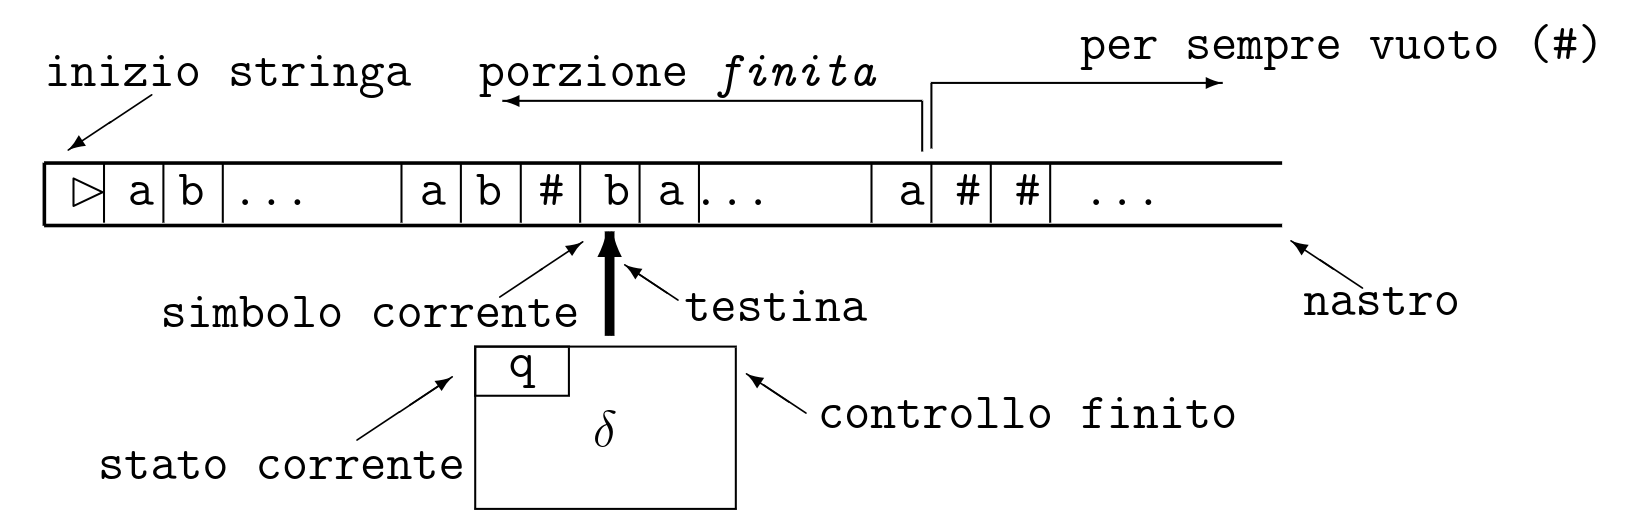
\includegraphics[scale=0.225]{images/turing.png}
\end{center}
Tenendo a mente questa figura possiamo provare a costruire la
nostra prima MdT.

\begin{example} \label{ex: 11}
	Vogliamo costruire una MdT in grado di dirci se la stringa
	binaria in input contiene una sottosequenza composta da
	due $1$ consecutivi.

	Per costruire la nostra macchina abbiamo bisogno di due
	stati ($q_0$ e $q_1$), di due simboli ($0$ e $1$) e di
	una funzione di transizione $\delta$.

	Per capire se la stringa in input contiene almeno una
	sottostringa composta da due $1$ consecutivi, iniziamo
	con lo stato iniziale $q_0$, il quale indica sia lo stato
	inziale della macchina sia lo stato in cui la macchina
	deve transire ogni qual volta incontra uno $0$.

	Abbiamo poi bisogno di uno stato $q_1$ in cui la macchina
	transisce quando incontra un $1$ nella sequenza dopo essere
	stata in uno stato $q_0$.

	Se ci troviamo nello stato $q_1$ e incontriamo un altro $1$
	la macchina transisce nello stato $h$ di terminazione. La
	funzione $\delta$ di transizione che deriva dai seguenti
	ragionamenti è la seguente
	\begin{center}
		\begin{tabular}{|c|c|c|}
			\hline
			$q$   & $\sigma$ & $\delta(q, \sigma)$ \\
			\hline
			$q_0$ & $\start$ & $q_0, \start, R$    \\
			$q_0$ & $0$      & $q_0, \#, R$        \\
			$q_0$ & $1$      & $q_1, \#, R$        \\
			$q_1$ & $0$      & $q_0, \#, R$        \\
			$q_1$ & $1$      & $h, \#, -$          \\
			\hline
		\end{tabular}
	\end{center}
	Come possiamo notare, ogni volta che incontriamo un
	carattere lo "cancelliamo" scrivendo $\#$ ma avremmo potuto
	lasciare il numero che incontravamo. Vediamo una possibile
	simulazione di esecuzione con la seguente stringa binaria
	in input
	\[ 01011 \]
	La nostra configurazione iniziale è
	\[ q_0 / \underline{\start} 01011 \]
	dove il simbolo sottolineato è quello su cui si trova il
	cursore. La sequenza di operazioni sarà quindi la seguente
	\begin{align*}
		q_0 / & \underline{\start} 01011       \\
		q_0 / & \start \underline{0} 1011      \\
		q_0 / & \start \# \underline{1} 011    \\
		q_1 / & \start \#\# \underline{0} 11   \\
		q_0 / & \start \#\#\# \underline{1} 1  \\
		q_1 / & \start \#\#\#\# \underline{1}  \\
		h /   & \start \#\#\#\# \underline{\#}
	\end{align*}
	Il calcolo è dunque terminato con successo.
\end{example}

Per vedere una MdT in azione è possibile visitare questo
\href{https://turingmachinesimulator.com/}{sito} in cui è
possibile programmare una MdT oppure eseguire esempi già
proposti.

\subsection{Configurazione e computazione}
Come abbiamo detto precedentemente, una \textbf{configurazione}
è definita dalla quadrupla
\[ \gamma = (q, u, \sigma, v) \]
Ciò che non abbiamo detto è che gli elementi di $\gamma$
appartengono al seguente insieme
\[
	\gamma \in (Q \cup \{ h \}) \times
	\Sigma^* \times \Sigma \times \Sigma^F
\]
L'ultimo insieme ($\Sigma^F$) è un po' particolare, è infatti
definito come
\[
	\Sigma^F = \Sigma^* \cdot \left( \Sigma \backslash
	\{ \# \} \right) \cup \{ \epsilon \}
\]
quindi possiamo scrivere la stringa $v$ come
$\sigma_0 \sigma_1 \dots \sigma_n$, con $\sigma_n \neq \#$,
al posto della stringa infinita composta dai vari $\sigma$ e
con infiniti $\#$ alla fine.

Si noti però che un qualsiasi carattere $\sigma_i$ con $i < n$
può essere $\#$ ed inoltre la stringa $u$ può essere vuota
solo quando il carattere corrente è $\start$. La convenzione
impone quindi di scrivere la configurazione iniziale del primo
esempio fatto, in questo modo
\[ (q_0, \start 01011, \epsilon) \]

\begin{definition}
	Una \textbf{computazione} è una successione finita di
	passi
	\[ (q_0, w) \to^* (q', w') \]
	dove $\to^*$ è la chiusura riflessiva e transitiva di
	$\to$. Ovviamente se vi sono $n$ passi, la computazione
	è lunga $n$ e dunque scriveremo $\to^n$.
\end{definition}

Definiamo meglio cos'è un \textbf{passo di computazione},
procedendo per casi e considerando $a$, $b$ e $c$ come elementi
generici di $\Sigma$.
\begin{itemize}
	\item $(q, u \underline{a} v) \to (q', u \underline{b} v)$
	      se $\delta (q, a) = (q', b, -)$.
	\item $(q, u c \underline{a} v) \to
		      (q', u \underline{c} b v)$
	      se $\delta (q, a) = (q', b, L)$.
	\item \begin{enumerate}
		      \item $(q, u \underline{a} c v) \to
			            (q', u b \underline{c} v)$
		            se $\delta (q, a) = (q', b, R)$.
		      \item $(q, u \underline{a}) \to
			            (q', u b \underline{\#})$
		            se $\delta (q, a) = (q', b, R)$.
	      \end{enumerate}
\end{itemize}
In questo modo garantiamo che ciascun passo abbia effetto
limitato sulle configurazioni, come richiesto dalla seconda
parte del punto 2 nell'\hyperref[sec: algoritmo]{idea intuitiva
	dell'algoritmo}.

Allo stesso modo possiamo immaginarci che se partiamo da uno
stato iniziale $(q_0, \underline{\start} w)$, dopo un certo
numero di passi arriviamo in uno stato $(q', w')$.

\begin{definition} \label{def: convergenza}
	Diciamo che una computazione \textbf{termina} o
	\textbf{converge} ($\downarrow$) se e solo se lo stato
	finale è $h$. Nell'esempio \ref{ex: 11} fatto qui sopra
	$q' = h$.

	Diciamo invece che la computazione \textbf{non termina}
	o \textbf{diverge} ($\uparrow$) se e solo se per ogni
	$q'$ e $w'$ tali che
	\[ (q_0, w) \to^* (q', w') \]
	esistono $q''$ e $w''$ tali che
	\[ (q', w') \to^* (q'', w'') \]
	ovvero tali che è sempre possibile fare un nuovo passo di
	computazione.
\end{definition}

Come possiamo vedere, le MdT definite in questo modo,
rispettano l'idea intuitiva di algoritmo che abbiamo dato
all'inizio.

\begin{example} \label{ex: non termina}
	Facciamo un esempio di computazione che non termina mai
	tramite una macchine che semplicemente non contiene il
	simbolo $h$ di terminazione.
	\begin{center}
		\begin{tabular}{|c|c|c|}
			\hline
			$q$   & $\sigma$ & $\delta$             \\
			\hline
			$q_0$ & $\start$ & $q_0$, $\start$, $R$ \\
			$q_0$ & $a$      & $q_0$, $a$, $R$      \\
			$q_0$ & $\#$     & $q_0$, $\#$, $R$     \\
			\hline
		\end{tabular}
	\end{center}
\end{example}

Proviamo ora a fare un esempio più concreto di una MdT che
calcola qualcosa di più sensato rispetto agli esempi visti
fino ad ora.

\begin{example}
	Questa MdT si propone di calcolare la somma di due numeri
	$n$ ed $m$, dove $n$ ed $m$ sono rappresentati in notazione
	unaria tramite il simbolo $|$ ripetuto $n$ (o $m$) volte.
	La funzione $\delta$ è definita dalla seguente tabella
	\begin{center}
		\begin{tabular}{|c|c|c|}
			\hline
			$q$   & $\sigma$ & $\delta$         \\
			\hline
			$q_0$ & $\start$ & $q_0, \start, R$ \\
			$q_0$ & $|$      & $q_0, |, R$      \\
			$q_0$ & $+$      & $q_1, |, R$      \\
			$q_1$ & $|$      & $q_1, |, R$      \\
			$q_1$ & $\#$     & $q_2, \#, L$     \\
			$q_2$ & $|$      & $h, \#, -$       \\
			\hline
		\end{tabular}
	\end{center}
	Il simbolo $+$ deve essere tra le due sequenze di $|$.
	Proviamo ora ad eseguire la computazione per il calcolo
	di $1 + 2$, partendo dalla configurazione iniziale
	\[ q_0/ \quad \underline{|} + | | \]
	Svolgiamo quindi i seguenti passi
	\begin{gather*}
		(q_0, \; \underline{\start} | + | | ) \to
		(q_0, \; \start \underline{|} + | | ) \\
		(q_0, \; \start \underline{|} + | | ) \to
		(q_0, \; \start | \underline{+} | | ) \\
		(q_0, \; \start | \underline{+} | | ) \to
		(q_1, \; \start | | \underline{|} | ) \\
		(q_1, \; \start | | \underline{|} | ) \to
		(q_1, \; \start | | | \underline{|} ) \\
		(q_1, \; \start | | | \underline{|} ) \to
		(q_1, \; \start | | | | \underline{\#} ) \\
		(q_1, \; \start | | | | \underline{\#} ) \to
		(q_2, \; \start | | | \underline{|} \# ) \\
		(q_2, \; \start | | | \underline{|} \# ) \to
		(h, \; \start | | | \underline{\#} \# )
	\end{gather*}
	per concludere che il calcolo termina dato che siamo
	giunti nello stato speciale $h$. Come possiamo vedere il
	nostro risultato è dato dal numero di $|$ rimanente.
\end{example}

Un altro tipico esempio di utilizzo di queste macchine è
quello di decidere se una stringa è palindroma. In questo
caso descriviamo brevemente quale sarebbe l'idea.
\begin{enumerate}
	\item Si controlla il primo carattere della stringa, lo si
	      sovrascrive con $\start$ e si passa in uno stato
	      specifico per quel carattere (supponendo che il primo
	      carattere sia $a$, si passa in $q_a$).
	\item Si arriva in fondo alla stringa e si controlla che
	      l'ultimo carattere sia uguale al primo, se sì, lo
	      si sovrascrive con un $\#$.
	\item Si torna indietro fino al primo $\start$ che si
	      incontra.
\end{enumerate}
Si ripete il procedimento finché non si esaurisce tutta la
stringa o finché non fallisce.

\chapter{Linguaggi FOR e WHILE}
Introduciamo ora un formalismo sicuramente a noi più familiare,
che è quello di un semplice linguaggio \textbf{imperativo} e
che quindi riesce ad esprimere i concetti di \textbf{memoria}
e di \textbf{comando}.

\section{Sintassi astratta}
La sintassi proposta è \emph{ambigua}, abbiamo dunque diverse
possibili interpretazioni per la stessa stringa. In realtà
tale sintassi viene elaborata tramite alberi, che hanno proprio
il compito di eliminare eventuali ambiguità.

Come vedremo a breve si tratta di una sintassi molto semplice,
comprendente costrutti condizionali di base, la possibilità
di eseguire cicli e semplici operazioni aritmetiche e logiche.

\begin{align*}
	E \to                                                 &
	\; n \; | \; x \; | \; E_1 + E_2 \; | \;
	E_1 \times E_2 \; | \; E_1 - E_2
	                                                      &
	\text{Espressioni aritmetiche}                          \\
	B \to                                                 &
	\; b \; | \; E_1 < E_2 \; | \; \lnot B \; | \;
	B_1 \lor B_2
	                                                      &
	\text{Espressioni booleane}                             \\
	C\to                                                  &
	\; \text{skip} \; | \; x := E \; | \; C_1 ; C_2 \; | \;
	\text{if } B \text{ then } C_1 \text{ else } C_2 \; | &
	\text{Comandi}                                          \\ &
	\; \text{for } x = E_1 \text{ to } E_2 \text{ do } C \; |
	\; \text{while } B \text{ do } C
\end{align*}

dove $n \in \N$, $x \in \Var$ (insieme numerabile di
variabili) e $b \in \text{Bool} = \{ tt, ff \}$.

D'ora in poi chiameremo \verb|WHILE|, il linguaggio descritto
dalla grammatica BNF di sopra. Chiameremo invece \verb|FOR|,
il linguaggio risultante dall'omissione del comando \verb|while|
della stessa grammatica.


\section{Semantica}
Prima di addentrarci nelle dinamiche del linguaggio appena
definito, dobbiamo definire la \textbf{memoria}. Nel nostro
caso lo facciamo tramite la funzione
\[ \sigma : \Var \to \N \]
che, data una variabile in input, restituisce il suo valore
in memoria (operazione di lettura). Noi però siamo interessati
anche a modificare la memoria, definiamo quindi l'operazione
di \textbf{aggiornamento} tramite la funzione, o meglio il
funzionale a tre argomenti
\[
	- [ - / - ] : (\Var \to \N) \times
	\N \times \Var \to (\Var \to \N)
\]
che è definita come
\[
	\sigma [n / x](y) = \begin{cases}
		n         & \text{se } y = x  \\
		\sigma(y) & \text{altrimenti}
	\end{cases}
\]
e cambia il valore della variabile $x$ con $n$. Quando
cercheremo di accedere nuovamente alla variabile $x$ in
memoria, la funzione $\sigma$ ci ritornerà il valore aggiornato.

La \textbf{semantica} di un'espressione aritmetica è data
dalla seguente funzione di \textbf{valutazione}, in cui andremo
a scrivere il suo argomento principale, l'espressione aritmetica,
tra le parentesi $[[$ e $]]$, cui viene giustapposto il secondo
argomento, cioè la memoria in cui l'espressione va valutata.
\[ \xi [[-]] - : E \times (\Var \to \N) \to \N \]
Proviamo a capire come questa funzione si comporta quando
prende in input espressioni aritmetiche.
\begin{align*}
	\xi [[n]] \sigma              & = n         \\
	\xi [[x]] \sigma              & = \sigma(x) \\
	\xi [[E_1 + E_2]] \sigma      &
	= \xi [[E_1]] \text{ più } [[E_2]] \sigma   \\
	\xi [[E_1 \times E_2]] \sigma &
	= \xi [[ E_1 ]] \text{ per } [[E_2]] \sigma \\
	\xi [[E_1 - E_2]] \sigma      &
	= \xi [[ E_1 ]] \text{ meno } [[E_2]] \sigma
\end{align*}
Per adesso limitiamoci a notare che se diamo alla funzione di
valutazione un numero $n$, qualunque sia la memoria, questa
ci restituirà il numero stesso.

Se invece gli passiamo una variabile, questa ci restituirà
il valore della variabile in memoria, si fa infatti uso della
funzione $\sigma$.

Se invece passiamo una qualche operazione aritmetica, questa
verrà valutata come la somma (oppure sottrazione o prodotto)
delle valutazioni degli operandi.

\begin{example}
	Proviamo a valutare l'espressione
	\[ x \times 2 - ((y - 7) + 1) \]
	nella memoria $\sigma$ tale che
	\[ \sigma (x) = 3 \quad \text{e} \quad \sigma(y) = 5 \]
	I passaggi per risolvere l'esercizio sono i seguenti
	\begin{align*}
		  & \xi [[ x \times 2 - ((y - 7) + 1) ]] \sigma \\
		= & \xi [[ x \times 2 ]] \sigma \text{ meno }
		\xi [[ (y - 7) + 1 ]] \sigma
	\end{align*}
	come possiamo notare, quando c'è un'ambiguità tra le
	precedenze supponiamo di sapere quale sia l'ordine
	corretto. In questo caso valutiamo "prima" il meno.
	\begin{align*}
		= & (\xi [[ x ]] \sigma \text{ per } 2) \text{ meno }
		\xi [[ (y - 7) + 1 ]] \sigma                          \\
		= & (\sigma(x) \text{ per } 2) \text{ meno }
		\xi [[ (y - 7) + 1 ]] \sigma                          \\
		= & (3 \text{ per } 2) \text{ meno }
		\xi [[ (y - 7) + 1 ]] \sigma
	\end{align*}
	ora abbiamo semplicemente preso il valore $3$ dalla memoria
	per sostituirlo a $x$.

	\begin{align*}
		= & 6 \text{ meno } (\xi [[y - 7]] \sigma
		\text{ più } 1)                                  \\
		= & 6 \text{ meno } ((\xi [[y]] \text{ meno } 7)
		\text{ più } 1)                                  \\
		= & 6 \text{ meno } ((\sigma(y) \text{ meno } 7)
		\text{ più } 1)
	\end{align*}
	Di seguito $5 - 7 = 0$ perché stiamo utilizzando il
	\emph{meno ridotto}, il quale ritorna $0$ quando il
	minuendo è maggiore o uguale del sottraendo.
	\begin{align*}
		= & 6 \text{ meno } ((5 \text{ meno } 7)
		\text{ più } 1)                          \\
		= & 6 \text{ meno } (0 \text{ più } 1)   \\
		= & 6 \text{ meno } 1 = 5
	\end{align*}
	Il calcolo per il resto è abbastanza banale.
\end{example}

Passiamo ora alla semantica delle operazioni booleane, che
non si inventano nulla di diverso rispetto alle espressioni
aritmetiche. Semplicemente la funzione di valutazione è
definita in modo da restituire valori booleani.
\[ \B[[-]] - : \B \times (\Var \to \N) \to \text{Bool} \]
Come prima andiamo a vedere cosa succede per vari input a
tale funzione di valutazione.
\begin{align*}
	\B [[t]] \sigma            & = tt                           \\
	\B [[f]] \sigma            & = ff                           \\
	\B [[E_1 < E_2]] \sigma    & =
	\xi [[E_1]] \sigma \text{ minore } \xi [[E_2]] \sigma       \\
	\B [[\lnot B]] \sigma      & = \text{ not } \B [[B]] \sigma \\
	\B [[B_1 \lor B_2]] \sigma & = \B [[B_1]] \sigma
	\text{ or } \B [[B_2]] \sigma
\end{align*}
Lo stile di definizione seguito fino ad ora prende il nome di
stile \textbf{denotazionale} e si propone di associare una
funzione a ciascun operatore.

Ci sono vari modi per definire una semantica, noi per il
momento andremo a definire la semantica tramite un approccio
\textbf{operazionale}, ossia guidato dalla sintassi.

Quello che andremo a fare è definire una sorta di macchina
astratta che procede per passi discreti, apportando modifiche
discrete alle sue configurazioni o stati, che possiamo
immaginare come coppie $(\text{comando}, \sigma)$.

Tale macchina, che definisce la semantica di un linguaggio
di programmazione, prende il nome di
\text{sistema di transizioni} ed è identificato dalla coppia.
\[ (\Gamma, \to) \]
dove $\Gamma$ è la classe delle \emph{configurazioni} (nel
nostro caso sono coppie $(C, \sigma)$) e
$\to \subseteq \Gamma \times \Gamma$ è una funzione detta
\textbf{di transizione}.

Tale coppia definisce come il nostro programma evolve in base
ai comandi che dobbiamo eseguire e a come questi modificano
la memoria.

In realtà noi seguiremo un approccio di tipo
\textbf{Structural Operational Semantics} (o
\emph{small steps}), in cui ciascuna transizione
\[ (c, \sigma) \to (c', \sigma') \]
rappresenta un singolo passo di computazione, ossia la macchina
ha attraversato lo stato $(c, \sigma)$ e \emph{transisce} nello
stato $(c', \sigma')$.

Possiamo allora fare considerazioni del tutto analoghe a quelle
fatte per la MdT, ossia possiamo dire che una computazione è
la chiusura riflessiva e transitiva della funzione di
transizione. Formalmente
\[ (c, \sigma) \to^* (c', \sigma') \]
In questo caso una computazione termina (o converge) se
\[ (c, \sigma) \to^* \sigma' \]
Quello che si vuole è che la relazione descritta precedentemente
come \emph{passo di computazione} soddisifi i seguenti assiomi
e regole di inferenza
\begin{center}
	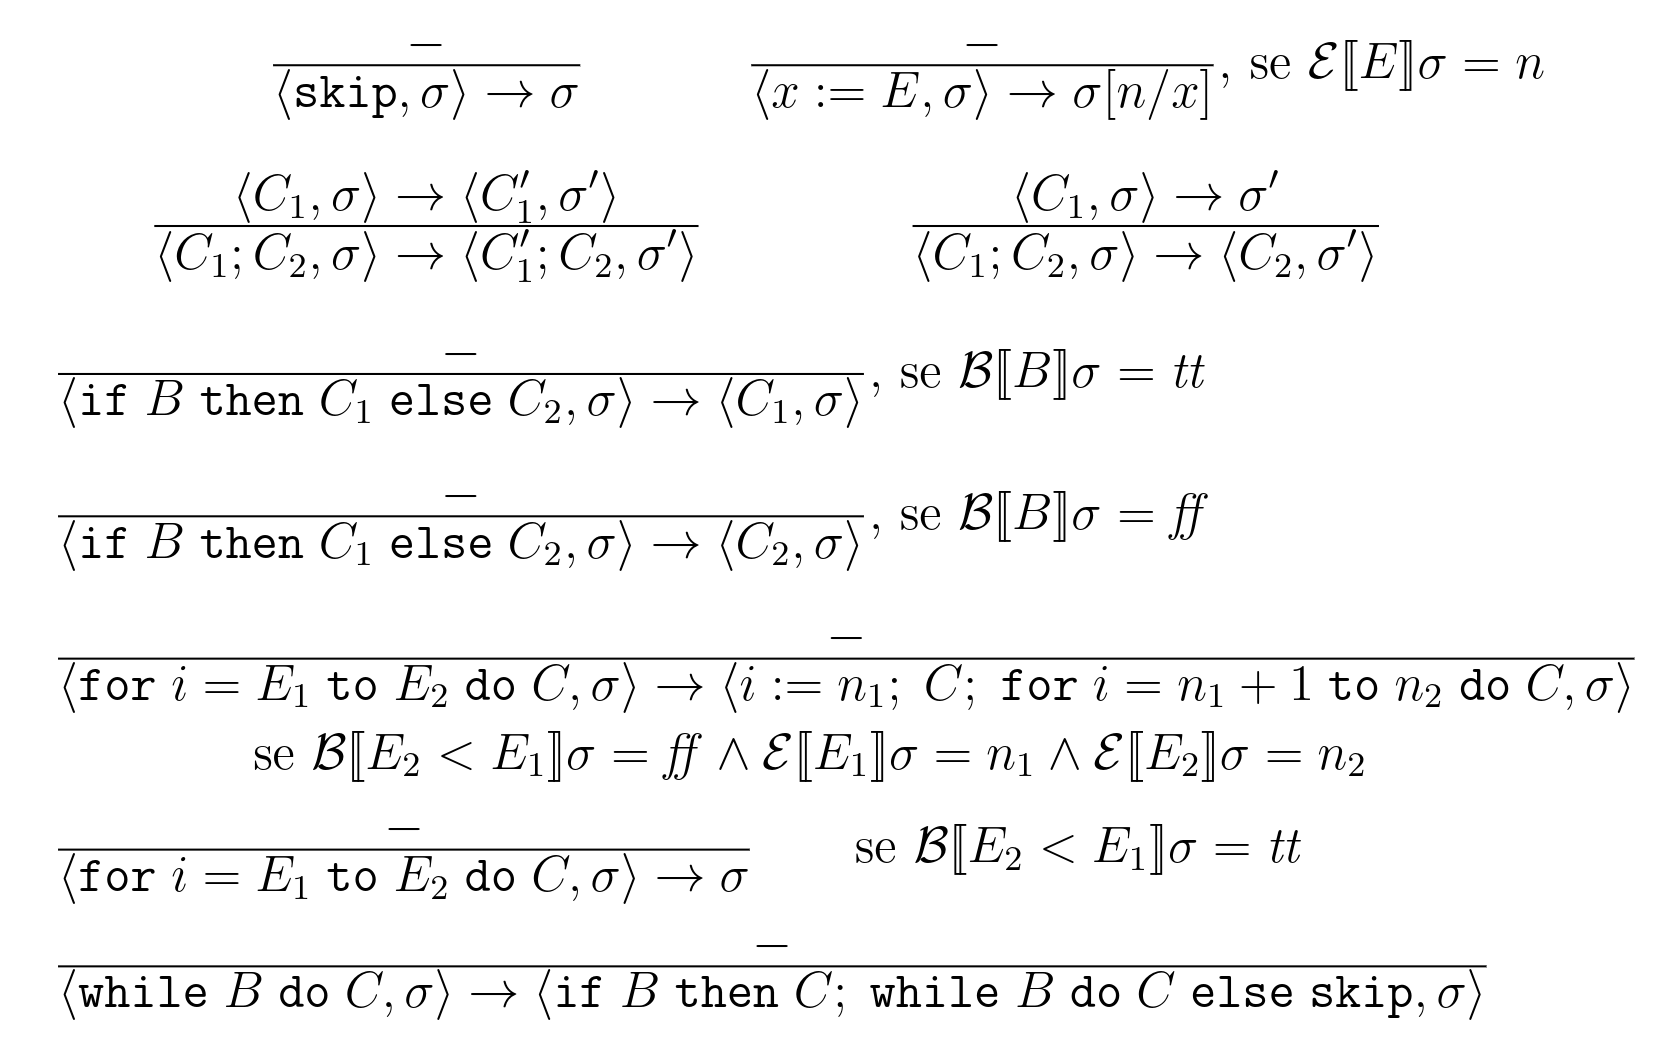
\includegraphics[scale=0.225]{images/assiomi.png}
\end{center}
Di particolare interesse è la regola di inferenza per
l'assegnamento, poiché chiarisce l'operazione di
\emph{aggiornamento} della memoria che avevamo lasciato in
sospeso.

Noi ci comportiamo come se la memoria fosse già inizializzata
per il nostro programma. Non ci sono vere e proprie operazioni
di scrittura della memoria. Ogni variabile esiste già in
essa e l'unica che cosa che ci è concesso fare è modificare il
suo valore.

Con la notazione $\sigma[n/x]$ intendiamo modificare il valore
della variabile $x$ presente in memoria con $n$. Stiamo in
realtà modificando la funzione che associa a $x$ un certo
valore (supponiamo $m$) con un altro valore ($n$).

La notazione che avevamo visto in precedenza per l'operazione
di aggiornamento significa che, se diamo $y$ in input a
$\sigma$ modificata, ossia $\sigma [n / x]$, se $y = x$,
allora stiamo in realtà cercando il valore di $x$ e dunque la
funzione ritorna $n$. Altrimenti stiamo cercando il valore di
$y$ presente in memoria e mai modificato dall'inizio
dell'esecuzione.

Per le altre regole teniamo a mente che, tutte quelle che
presentano una condizione a destra, si potrebbero scrivere
con la stessa condizione sopra.

In ogni caso per leggere le regole di inferenza seguiamo un
patter di questo tipo: se ci troviamo nello stato definito
descritto sotto la riga e a sinistra della freccia, si
transisce nello stato a destra della freccia se la condizione
è verificata.

\begin{example}
	Proviamo a dimostrare che il comando $C_1 ; C_2$ termina,
	tramite induzione.
	\begin{proof}
		Partiamo dalla regola di inferenza
		\[
			\frac{(C_1, \sigma) \to \sigma'}
			{(C_1 ; C_2, \sigma) \to (C_2 , \sigma')}
		\]
		e come ipotesi induttiva usiamo il fatto che se
		$C_1$ termina e $C_2$ termina, allora $C_1 ; C_2$
		termina. Se consideriamo la regola di inferenza
		\[
			\frac{(C_1, \sigma) \to (C_1', \sigma')}
			{(C_1 ; C_2, \sigma) \to (C_1' ; C_2 , \sigma')}
		\]
		il discorso è analogo con un passaggio in più. Se
		$C_1'$ termina ci ritroviamo al caso precedente e
		quindi anche $C_1 ; C_2$ termina.
	\end{proof}
\end{example}

\begin{example}
	Proviamo invece a dimostrare che il seguente programma
	\[ \text{while } tt \text{ do} \text{ skip}, \sigma \]
	non termina.
	\begin{proof}
		Per dimostrare che il programma non termina iniziamo
		a prendere la nostra configurazione di comandi e
		notiamo che corrisponde alla regola
		\[
			\frac{-}{(\text{while } B \text{ do } C, \sigma)
				\to (\text{if } B \text{ then } C;
				\text{ while } B \text{ do } C
				\text{ else skip}, \sigma )}
		\]
		che ci fa transire nello stato
		\[
			\text{if } tt \text{ then skip}, \sigma;
			\text{ while } tt \text{ do skip}, \sigma
			\text{ else skip}, \sigma
		\]
		a questo punto usiamo l'assioma dell'\verb|if| e
		otteniamo
		\[
			\text{skip}, \sigma ; \text{ while } tt
			\text{ do skip}, \sigma
		\]
		il primo comando è uno \verb|skip| e dunque ritorniamo
		al punto di partenza, ossia
		\[ \text{while } tt \text{ do} \text{ skip}, \sigma \]
		Ne concludiamo quindi che siamo entrati in un ciclo
		infinito.
	\end{proof}
\end{example}


\chapter{Problemi e funzioni}
Per il momento abbiamo usato i nostri costrutti per calcolare
una funzione (la somma per esempio) o per decidere
l'appartenenza di un elemento ad un insieme (decidere se una
stringa è palindroma).

In questa prima parte del corso andremo a definire meglio il
concetto di \textbf{problema} e di \textbf{funzione} che, nel
nostro caso, non hanno l'accezione cui siamo abituati.

Un esempio di \emph{problema} è la domanda: "qual è il massimo
comun divisore tra $x$ e $y$?". Se sostituiamo a $x$ e a $y$
dei valori, per esempio 34 e 98, otteniamo un \textbf{caso}
del problema.

\begin{definition} \label{def: T-calcolabile}
	Siano $\Sigma$, $\Sigma_0$ e $\Sigma_1$ tali che
	\[ \#, \start \notin \Sigma_0 \cup \Sigma_1 \]
	e
	\[ \Sigma_0 \cup \Sigma_1 \subset \Sigma \]
	allora diciamo che una funzione
	\[ f : \Sigma_0 \to \Sigma_1 \]
	è \textbf{Turing calcolabile} o \textbf{T-calcolabile},
	se e solo se
	\begin{gather*}
		\forall w \in \Sigma_0^* : f(w) = z \\
		\Updownarrow \\
		(q_0, \underline{\start} w) \to_M^*
		(h, \start z \underline{\#})
	\end{gather*}
	Si dice anche che $f$ è T-calcolabile se esiste una MdT
	$M$ che la calcola.
\end{definition}

Ora che abbiamo la definizione precisa di cosa sia una
funzione T-calcolabile proviamo a fare una cosa analoga per
il linguaggio WHILE che abbiamo definito in precedenza.

\begin{definition} \label{def: while-calcolabile}
	Diciamo che una funzione
	\[ f : \Var \to \N \]
	è \textbf{WHILE-calcolabile} oppure diciamo che un comando
	$C$ \textbf{calcola} $f$, se e solo se
	\begin{gather*}
		\forall \sigma \in \Var \to \N : f(x) = n \\
		\Updownarrow \\
		(C, \sigma) \to^* \sigma' \quad \land \quad
		\sigma'(x) = n
	\end{gather*}
\end{definition}

Notiamo che la variabile $x$ di input è anche la variabile
di output, ossia quella che contiene il risultato.


\section{Codifiche}
Ci chiediamo ora se per una funzione $f$ che non opera su
dati sotto formato di stringa, memorie o numeri naturali,
le nozioni di calcolabilità che abbiamo definito fino ad ora
sono ancora valide.

Se così non fosse dovremmo ridefinire ogni volta tali nozioni
per ogni dominio di ogni funzione con un formato differente da
quelli che abbiamo già incontrato.

Per superare il problema si fa uso di opportune
\textbf{codifiche} dei dati, ossia funzioni che svolgono
il seguente compito.
\begin{enumerate}
	\item Dato $x$ in formato $A$, lo si codifica in un formato
	      $B$ che ci permette di effettuare il calcolo con un
	      formalismo che conosciamo, per esempio le MdT e
	      otteniamo $y$.
	\item Si applica la MdT a $y$ e si ottiene il risultato $z$
	      (se la computazione termina) in formato $B$.
	\item Si traduce $z$ dal formato $B$ al formato $A$.
\end{enumerate}
D'ora in avanti considereremo solo i numeri naturali come i
nostri dati. Abbiamo però bisogno che la funzione di codifica
sia \emph{biunivoca}.

\begin{example}
	La seguente funzione codifica coppie di naturali come un
	singolo naturale ed è detta codifica a
	\textbf{coda di colomba}.
	\[ (x, y) \to \frac{1}{2} (x^2 + 2 x y + y^2 + 3 x + y) \]
	la cui decodifica, ossia la funzione inversa è la seguente
	\[
		n \to (n - \frac{1}{2} k \cdot (k + 1),
		k - (n - \frac{1}{2} k \cdot (k + 1))
	\]
	dove $k=\lfloor \frac{1}{2}(\sqrt{1+8\cdot n}-1)\rfloor$.
\end{example}

Possiamo quindi dire che le proprietà basilari dei formalismi
e delle classi di funzioni calcolate, non cambiano al variare
del formato dei dati su cui operano.

\begin{definition} \label{def: funzione totale}
	Diciamo che una funzione $f : A \to B$, sottoinsieme di
	$A \times B$ è una \textbf{funzione totale} se e solo se
	\begin{itemize}
		\item \`E \emph{definita ovunque}, ossia se
		      $\forall a \in A$, $\exists b \in B$ tale che la
		      coppia $(a, b) \in f$.
		\item Vi è \emph{unicità}, ossia se, date le coppie
		      $(a, b) \in f$ e $(a, c) \in f$, allora $b=c$.
	\end{itemize}
	Una funzione totale è quindi suriettiva ma potrebbe non
	essere iniettiva.
\end{definition}

Una funzione può essere calcolabile ma non totale, per esempio
la macchina di Turing che non termina mai vista nell'esempio
\ref{ex: non termina}.

\begin{definition} \label{def: funzione parziale}
	Diciamo che una funzione $f : A \to B$ è \textbf{parziale}
	se è un sottoinsieme di $A \times B$ tale che
	\begin{itemize}
		\item Vi è \emph{unicità}, ossia se, date le coppie
		      $(a, b) \in f$ e $(a, c) \in f$, allora $b = c$.
		\item Esiste al più un $b \in B$ tale che $f(a) = b$.
	\end{itemize}
	e quindi non si richiede che $f$ sia definita ovunque.
\end{definition}

Introduciamo ora un po' di notazione utile a quello che faremo
più avanti. Data una funzione $f : A \to B$
\begin{itemize}
	\item Diremo che $f$ è \textbf{definita} o
	      \textbf{converge su $a$} ($f(a) \downarrow$) se
	      $\exists b$ tale che $(a, b) \in f$ (cioè
	      $f(a) = b$).
	\item Diremo che $f$ \textbf{non è definita} o che
	      \textbf{diverge} ($f(a) \uparrow$) se $\nexists b$
	      tale che $(a, b) \in f$.
\end{itemize}
Chiamiamo inoltre
\begin{itemize}
	\item \textbf{Dominio} di $f$ l'insieme
	      \[ \{ a \in A \; | \; f(a) \downarrow \} \]
	      che coincide con lo spazio di partenza ($A$) se e
	      solo se la funzione è totale.
	\item \textbf{Codominio} di $f$ l'insieme $B$.
	\item \textbf{Immagine} di $f$ l'insieme
	      \[ \{ b \in B \; | \; \exists a \in A : f(a) = b \} \]
	      Quando immagine e codominio coincidono abbiamo una
	      funzione suriettiva.
\end{itemize}

Detto questo vogliamo capire qual è la relazione tra funzioni
e algoritmi. Una funzione possiamo vederla come un insieme di
coppie (\emph{argomento}, \emph{risultato}) (o (\emph{input},
\emph{output}) se preferiamo la notazione più informatica) ma
non ci dice come il risultato (o l'output) venga calcolato.

Di conseguenza non ci sono due funzioni diverse che per uno
stesso argomento restituiscono lo stesso risultato. In termini
insiemistici possiamo dire che non esistono due insiemi diversi
che hanno gli stessi elementi.
\begin{tcolorbox}
	Un algoritmo è invece una \textbf{rappresentazione finita}
	di una funzione, in quanto specifica come si calcola il
	risultato a partire dall'argomento. In questo caso possiamo
	certamente avere più algoritmi che calcolano la stessa
	funzione.
\end{tcolorbox}
Per esempio possiamo scrivere infiniti programmi \verb|WHILE|
che calcolano la stessa funzione aggiungendo dei comandi
\verb|skip| ad ognuno di essi.

\section{Funzioni calcolabili}
D'ora in avanti proveremo a capire
\begin{itemize}
	\item Quali sono le \textbf{funzioni calcolabili} e di
	      quali proprietà godono.
	\item Se esistono funzioni totali o parziali che non sono
	      calcolabili. Ovvero per cui si dimostra che non esiste
	      un algoritmo che le calcoli.
\end{itemize}
Per farlo andremo a focalizzarci più sul concetto di funzione
rispetto al concetto di algoritmo andando quindi ad analizzare
\emph{cosa} si calcola e non \emph{come} lo si calcola.

\begin{example}
	Prendiamo ora come esempio la
	\textbf{congettura di Goldbach}, la quale ci dice che ogni
	numero pari maggiore di 2 è esprimibile come somma di due
	numeri primi. Da questa congettura (mai dimostrata) nasce
	la \textbf{funzione di Goldbach}, definita come segue con
	$gb : \N \to \N$
	\[
		gb(n) = \begin{cases}
			0 & \text{se la congettura è vera} \\
			1 & \text{altrimenti}
		\end{cases}
	\]
	La congettura non è stata ancora dimostrata ma un algoritmo
	per calcolarla esiste, solo che non sappiamo quale sia.

	Se ad esempio volessimo decidere se la funzione è
	T-calcolabile, basterebbe prendere una MdT che ritorna
	sempre 0 se la congettura è vera o una MdT che ritorna
	sempre 1 se è falsa. Il problema è che fin tanto che la
	congettura non è dimostrata, non sappiamo quale delle due
	scegliere.
\end{example}



\chapter{Funzioni ricorsive primitive}
Iniziamo con il definire due delle più popolari funzioni
definite per \emph{ricorrenza}: il fattoriale e la successione
di Fibonacci.

Iniziamo con il \emph{fattoriale}, definito come una coppia
di equazioni, la prima per il caso base, ossia quando $x = 0$
e la seconda per tutti gli altri casi, ossia per ogni $x > 0$.
\[
	\begin{cases}
		!(0)     & = 1                  \\
		!(x + 1) & = (x + 1) \cdot !(x)
	\end{cases}
\]
Proviamo a scrivere una versione \verb|WHILE| e una versione
\verb|FOR| del fattoriale
\begin{verbatim}
    fatt := 1;
    while x > 0 do
        fatt := fatt * x;
        x := x - 1;
\end{verbatim}
in questo caso salviamo il risultato nella variabile
\verb|fatt| che è la stessa che usiamo per ritornare il
risultato.

La \emph{successione di Fibonacci} presenta invece due casi
base e un caso definito per ricorrenza ed è definita come
segue
\[
	\begin{cases}
		fib(0)     & = 0                   \\
		fib(1)     & = 1                   \\
		fib(x + 2) & = fib(x + 1) + fib(x)
	\end{cases}
\]
Ora vogliamo capire quali sono le regole per formare bene
delle formule ricorsive ed è qui che prenderemo un po' di
notazione in prestito dal $\lambda$-calcolo. Nel caso del
fattoriale possiamo scrivere
\[ \lambda x . !(x) \]
per dire che il fattoriale dipende solo da $x$. Possiamo anche
scrivere un qualcosa di questo tipo
\[ \lambda x . x + y \]
per definire una funzione che prende $x$ e restituisce una
funzione che dipende da $y$. Abbiamo quindi un modo per
\emph{costruire} delle funzioni specificando esattamente quali
sono i suoi argomenti.

\begin{definition} \label{def: ricorsive primitive}
	Le \textbf{funzioni ricorsive primitive} sono la minima
	classe $\C$ da $\N^n$, con $n \geq 0$, in $\N$ cui
	appartengono le funzioni
	\begin{itemize}
		\item \textbf{Zero}: una funzione che prende $k \geq 0$
		      di argomenti e ritorna 0.
		      \[ \lambda x_1, \dots, x_k . 0 \]
		\item \textbf{Successore}: che prende un argomento solo
		      e restituisce il suo successore
		      \[ \lambda x . x + 1 \]
		\item \textbf{Identità}: che prende $k$ argomenti e
		      ritorna l'argomento $i$-esimo con $1\leq i\leq k$.
		      \[ \lambda x_1, \dots, x_k . x_i \]
		      Viene anche chiamata \textbf{proiezione}.
	\end{itemize}
	Questi sono anche detti \textbf{schemi primitivi di base}.
	La classe $\C$ che stiamo provando a definire è inoltre
	\emph{chiusa} per
	\begin{itemize}
		\item \textbf{Composizione}: Se $g_1, \dots, g_k \in \C$
		      sono funzioni in $m$ variabili, e $h \in \C$ è
		      una funzione in $k$ variabili, anche la loro
		      composizione
		      \[
			      \lambda x_1, \dots x_m .
			      h(g_1(x_1, \dots, x_m), \dots,
			      g_k(x_1, \dots, x_m)
			      )
		      \]
		      appartiene a $\C$.
		\item \textbf{Ricorsione primitiva}: Se $h \in \C$
		      è una funzione in $k+1$ variabili, $g \in \C$
		      è una funzione in $k-1$ variabili definita da
		      \[
			      \begin{cases}
				      f(0, x_2, \dots, x_k)       & =
				      g(x_2, \dots, x_k)              \\
				      f(x_1 + 1, x_2, \dots, x_k) & =
				      h(x_1, f(x_1, \dots, x_k),
				      x_2, \dots, x_k)
			      \end{cases}
		      \]
	\end{itemize}
\end{definition}

\begin{tcolorbox}
	Dato che $\C$ è la \emph{minima} classe che soddisfa le
	condizioni espresse sopra, affinché $f$ sia ricorsiva
	primitiva, occorre e basta che sia una successione finita,
	o \textbf{derivazione}, della seguente forma
	\[ f_1, \dots, f_n \]
	tale che $f = f_n$ e per ogni $i$ tale che
	$1 \leq i \leq n$ vale uno dei seguenti casi:
	\begin{itemize}
		\item $f_i \in C$ è una funzione di \emph{Zero} o è
		      l'\emph{Identità}.
		\item $f_i$ è ottenibile tramite l'applicazione delle
		      regole di \emph{Combinazione} e
		      \emph{Ricorsione primitiva} da $f_j$ con $j < i$.
	\end{itemize}
\end{tcolorbox}

Tra i requisiti necessari affinché una funzione venga definita
\emph{ricorsiva primitiva}, quello meno intuitivo tra quelli
descritti è sicuramente è quello che riguarda proprio la
ricorsione primitiva.

Come vediamo possiamo definire una funzione in funzione di se
stessa, ma con delle limitazioni. Abbiamo infatti un primo caso
in cui il primo argomento è $0$ e non c'è una chiamata
ricorsiva, siamo quindi davanti ad un caso base.

Più complesso è il secondo caso, in cui diciamo che la funzione
su $k$ argomenti ritorna il primo argomento decrementato, come
secondo argomento ha una chiamata ricorsiva su tutti gli
argomenti e il resto degli argomenti sono quelli che vanno dal
secondo al $k$-esimo e rimangono invariati.

\begin{example}
	Definiamo ora la somma tramite le regole appena descritte.
	\[
		\begin{array}{ll}
			f_1 & = \lambda x.x                    \\
			f_2 & = \lambda x.x + 1                \\
			f_3 & = \lambda x_1, x_2, x_3 . x_2    \\
			f_4 & = f_2 (f_3 (x_1, x_2, x_3))      \\
			f_5 & = \begin{cases}
				        f_5 (0, x_2)     & = f_1 (x_2) \\
				        f_5 (x + 1, x_2) & =
				        f_4 (x_1, f_5(x_1, x_2), x_2)
			        \end{cases}
		\end{array}
	\]
	Qui l'idea, avendo come unica funzione di somma la funzione
	successore, è quella di calcolare il successore del primo
	numero tante volte quanto è il secondo numero. A questo
	punto proviamo a calcolare $2 + 3$.
	\[
		\begin{array}{l}
			f_5(2, 3) =                         \\
			f_4 (1, f_5(1, 3), 3) =             \\
			f_4 (1, f_4(0, f_5 (0, 3), 3), 3) = \\
			f_4 (1, f_4(0, f_1 (3), 3), 3) =    \\
			f_4 (1, f_4(0, 3, 3), 3) =          \\
			f_4 (1, f_2(f_3(0, 3, 3)), 3) =     \\
			f_4 (1, f_2(3), 3) =                \\
			f_4 (1, 4, 3) =                     \\
			f_2 (f_3 (1, 4, 3)) =               \\
			f_2 (4) = 5
		\end{array}
	\]
\end{example}
Applicare la formula non è niente di difficile e forse
non è più di tanto istruttivo. Quello che ci interessa
principalmente è cosa sia una funzione ricorsiva primitiva e a
quali regole sottostare per definirne una.

Come abbiamo visto, siamo riusciti a definire la somma tramite
questo formalismo, ne segue che possiamo usarla per definire
anche il prodotto come ricorsiva primitiva. Possiamo ora
tornare alla formula con cui abbiamo definito il fattoriale
in precedenza, ossia
\[
	\begin{cases}
		!(0)     & = 1                  \\
		!(x + 1) & = (x + 1) \cdot !(x)
	\end{cases}
\]
che, come possiamo vedere, rispetta i vincoli necessari ad
essere una funzione ricorsiva primitiva in quanto abbiamo un
caso base in cui il primo (e unico) argomento è $0$. Abbiamo
inoltre un caso ricorsivo in cui si incrementa il primo
argomento di $1$ e si effettua una ricorsione (possiamo vedere
il prodotto come la funzione $h$ della definizione di ricorsione
primitiva).

\begin{definition} \label{def: relazione ricorsiva}
	Diciamo che la relazione $P(x_1, \dots, x_k) \subseteq \N^k$
	è \textbf{ricorsiva primitiva} se lo è la sua
	\textbf{funzione caratteristica} $\chi_P$, definita come
	\[
		\chi_P (x_1, \dots, x_k) = \begin{cases}
			1 & \text{se } (x_1, \dots, x_k) \in P \\
			0 & \text{altrimenti}
		\end{cases}
	\]
\end{definition}

Vediamo come esempio di relazione ricorsiva primitiva,
l'\textbf{uguaglianza}, definendo la sua funzione
caratteristica $\chi_=$ in questo modo
\begin{align*}
	\chi_= (0, 0)         & = 1             \\
	\chi_= (x + 1, y + 1) & = \chi_= (x, y) \\
	\chi_= (0, y + 1)     & = 0             \\
	\chi_= (x + 1, 0)     & = 0
\end{align*}
L'idea alla base è diminuire entrambi i valori di $1$ fino a
che uno dei due o entrambi sono sono $0$. Se uno solo dei due
vale $0$, allora non erano uguali, se entrambi sono $0$, allora
erano uguali.

Altre tre cose che ci servirà sapere sono che
\begin{itemize}
	\item $R = \{ x \in \N | x \text{ è un numero primo} \}$
	      è ricorsiva primitiva.
	\item \textbf{Teorema di unica fattorizzazione}: Se
	      $p_0 < \dots < p_k < \dots$ sono i numeri primi,
	      cioè $R = \{ p_0, \dots, p_k, \dots \}$, allora per
	      ogni $x \in \N$ esiste un numero finito di esponenti
	      $x_i \neq 0$ tali che
	      \[
		      x = p_0^{x_0} \cdot p_1^{x_1} \cdots
		      p_n^{x_n} \cdots
	      \]
	\item La funzione $(x)_i$ l'esponente dell'$i$-esimo
	      fattore $p_i$ della fattorizzazione di $x$ è
	      ricorsiva primitiva.
\end{itemize}
La conseguenza fondamentale del teorema è che ogni sequenza
di naturali può essere codificata come un singolo numero
\[
	n = p_0^{n_0 + 1} \cdot p_1^{n_1 + 1} \cdots
	p_k^{n_k + 1}
\]
ovvero come il prodotto di un numero finito di fattori (con
ogni $p_i$ che è un numero primo), e viceversa.

In altre parole stiamo dicendo che esiste un solo numero $n$
che, data una sequenza $n_0 n_1 \dots n_k$, verifica
l'uguaglianza
\[
	n = p_0^{n_0 + 1} \cdot p_1^{n_1 + 1} \cdots
	p_k^{n_k + 1}
\]
e viceversa. Questa è la base per dimostrare che le funzioni
di codifica sono ricorsive primitive.

\section{Teoremi principali}

% \subsection{Teorema di enumerazione}


\chapter{Diagonalizzazione}
Fino ad ora abbiamo visto che formalismi come programmi FOR
e funzioni ricorsive primitive calcolano \emph{solo} funzioni
totali. Ci chiediamo adesso se esiste un formalismo che esprime
tutte le funzioni calcolabili e per di più solo quelle totali.

La risposta è no e la \textbf{funzione di Ackermann} ne è un
esempio, la quale è totale ma non è ricorsiva primitiva.
Potremmo quindi pensare di estendere il formalismo per far sì
che anche questa funzione sia ricorsiva primitiva e chiederci
se a questo punto esiste un formalismo in grado di esprimere
tutte e sole le funzioni totali.

La risposta è ancora no e proveremo a dimostrarlo tramite un
metodo che prende il nome di \textbf{diagonalizzazione}. Questo
metodo, independente dal formalismo sul quale viene applicato,
a patto che quest'ultimo sia un formalismo con cui si possano
definire solo funzioni totali, permette di dimostrare che quel
formalismo non riesce ad esprimere tutte le funzioni calcolabili
totali in quanto ne manca almeno una che intuitivamente lo è.
\begin{enumerate}
	\item Ragioniamo in termini di funzioni ricorsive primitive
	      e chiamiamo quindi $f_n$ la funzione definita dalla
	      $n$-esima derivazione degli schemi primitivi di base.
	      Dato che le funzioni ricorsive primitive e le sue
	      possibili derivazioni sono stringhe finite prese da
	      un alfabeto finito, possiamo (ad esempio tramite il
	      processo di g\"odelizzazione) enumerarle.
	\item Definiamo la funzione
	      \[ g(x) = f_x(x) + 1 \]
	      che è una funzione calcolabile e totale in quanto
	      $f_x$ è l'$x$-esima derivazione di una funzione
	      ricorsiva primitiva.
	\item Ci si rende conto che $g$ non si trova nelle lista
	      delle funzioni ricorsive primitive perché $\forall x$
	      vale che
	      \[ g(x) = f_x(x) + 1 \]
	      e quindi $\forall x$ vale che
	      \[ g(x) \neq f_x(x) \]
	      In altre parole la funzione $g$ usa l'$x$-esima
	      funzione nella lista, gli applica $x$ e ci somma $1$,
	      ma l'$x$-esima funzione nella lista ritorna un
	      certo risultato $y$ e non $y + 1$.
\end{enumerate}
Ecco che la funzione $g$, che sicuramente è totale e calcolabile
non appartiene alla lista che abbiamo definito, in particolare
nel nostro caso non è una funzione ricorsiva primitiva.

Dato che la lista di tutte le $f_x$ è la lista di tutte le
funzioni ricorsive primitive e dato che
\[ g(x) \neq f_x (x) \]
siamo sicuri che $g$ non appartenga alla lista poiché è
sicuramente diversa da ogni funzione precedentemente enumerata.

Altro fatto da considerare è che, dato che $\forall x$ abbiamo
che $f_x$ è una funzione ricorsiva primitiva, è calcolabile e
totale. Se la funzione $g$ somma $1$ a $f_x$ non cambia il fatto
che sia anch'essa ricorsiva primitiva e dunque calcolabile e
totale. Non appartiene però alla lista delle funzioni
precedentemente enumerate.

\section{Diagonalizzazione per funzioni parziali}
A questo punto non ci rimane che capire se i formalismi che
abbiamo definito fino ad ora possono esprimere almeno tutte
le funzioni parziali calcolabili.

Come sappiamo dalla definizione \ref{def: funzione parziale}
le funzioni parziali non richiedono di essere definite ovunque
e questo ci tornerà comodo.

Cerchiamo quindi di dimostrare che la diagonalizzazione non si
applica anche a queste funzioni. Come prima possiamo enumerare
tutte le funzioni e prendere $\psi_n$, ossia l'$n$-esima
funzione nella lista, e applichiamo la diagonalizzazione.
Poniamo dunque
\[ \varphi (x) = \psi_x (x) + 1 \]
Supponiamo ora che $\varphi$ sia rappresentata dall'$n$-esimo
algoritmo: non possiamo tuttavia concludere che
\[ \varphi \neq \psi_n \]
perché $\psi_n(n)$ potrebbe non essere definita e dunque
divergere. Se $\psi_n(n)$ diverge, lo fa anche $\psi_n(n)+1$
e dunque le due funzioni sono equivalenti.

Le funzioni parziali, per fortuna, hanno senso, prendiamo ad
esempio la seguente funzione che definisce la divisione
\[ div (x,y) = \lfloor x / y \rfloor \]
che è definita solo se $y \neq 0$. Ci chiediamo quindi se sia
possibile estendere tutte le funzioni parziali a totali. Come
vedremo più avanti la risposta è no perché non sempre c'è un
algoritmo che calcola la versione estesa. Torniamo però al caso
della divisione. Se ad esempio definissimo accuratamente il
dominio della funzione, per esempio in questo modo
\[ div : \N \times \N \backslash \{ 0 \} \to \N \]
avremmo comunque il problema che non tutte le coppie di naturali
sono coperte. Introduciamo quindi un simbolo speciale
$* \notin \N$ in modo da avere ancora una funzione per tutte le
possibili coppie di naturali
\[ div^* : \N \times \N \to \N \cup \{ * \} \]
definita in questo modo
\[
	div^* (x, y) = \begin{cases}
		div(x, y) & \text{se } y \neq 0 \\
		*         & \text{se } y = 0
	\end{cases}
\]
Non vogliamo però liberarci della parzialità, dato che, come
abbiamo appena visto, la diagonalizzazione non funziona in
questo caso. Abbiamo quindi bisogno di un formalismo per
definire anche le funzioni parziali.


\chapter{Funzioni ricorsive generali}
Introduciamo ora le \textbf{funzioni ricorsive generali} come
un'estensione delle ricorsive primitive. In particolare vogliamo
aggiungere, agli schemi primitivi di base di \emph{combinazione}
e \emph{ricorsione primitiva} (\ref{def: ricorsive primitive}),
lo schema di \textbf{minimizzazione}.

Dobbiamo prima però introdurre un po' di notazione: l'operatore
$\mu$, detto \textbf{operatore di minimizzazione}, applicato
ad un insieme di numeri naturali, ne restituisce il minimo, se
presente.

\begin{definition} \label{def: mu ricorsive}
	La classe delle funzioni \textbf{$\mu$-ricorsive} (o
	\textbf{ricorsive generali}) è la minima classe
	$\RR$ tale che soddisfa le condizioni di
	\begin{itemize}
		\item \emph{Zero} e \emph{ricorsione primitiva}.
		\item \textbf{Minimizzazione}: se
		      $\varphi (x_1, \dots, x_n, y) \in \RR$ in $n+1$
		      variabili, allora la funzione $\psi$ in $n$
		      variabili è in $\RR$ se è definita dal minimo $y$
		      tale che
		      \begin{itemize}
			      \item $\varphi(x_1, \dots, x_n, y) = 0$
			      \item $\forall z \leq y$ vale $\varphi(x_1,
				            \dots, x_n, z) \downarrow$.
		      \end{itemize}
		      In forma più compatta la condizione di
		      minimizzazione è la seguente
		      \[
			      \psi (x_1, \dots, x_n) = \mu y [
					      \forall z \leq y, \;
					      \varphi(x_1, \dots, x_n, z)
					      \downarrow]
		      \]
	\end{itemize}
\end{definition}

Una funzione $\mu$-ricorsiva è intuitivamente calcolabile poiché
l'algoritmo \emph{intuitivo} che la calcola è composto da un
ciclo in cui si incrementa la variabile $y$ (inizialmente posta
a $0$), si calcola la $\varphi$ e si ripetono questi passi
finché il risultato non è $0$. I primi passi dell'esecuzione
di questo algoritmo potrebbero dunque essere:
\begin{enumerate}
	\item Calcolare $\varphi(x_1, \dots, x_n, 0)$. Se il
	      risultato è $0$, allora $\psi (x_1, \dots, x_n) = 0$.
	\item Altrimenti si calcola $\varphi(x_1, \dots, x_n, 1)$,
	      se il risultato è $0$, allora
	      $\psi(x_1, \dots, x_n)=1$.
	\item ...
\end{enumerate}
Intuitivamente l'algoritmo potrebbe non terminare mai perché
\begin{itemize}
	\item Per ogni valore di $y$ esiste un $m_y$ tale che
	      \[ \varphi (x_1, \dots, x_n, y) = m_y \neq 0 \]
	\item Per i primi $k$ numeri naturali vale che
	      \[
		      \varphi (x_1, \dots, x_n, z) = n_z \neq 0
		      \quad \land \quad
		      \varphi (x_1, \dots, x_n, k) \uparrow
	      \]
\end{itemize}
Nel primo caso infatti continuiamo a calcolare
$\varphi(x_1, \dots, x_n, y)$ per valori crescenti di $y$ senza
quindi terminare mai. Nel secondo caso non ci arrestiamo mai nel
calcolo di $\varphi (x_1, \dots, x_n, k) \uparrow$ poiché la
funzione diverge: da qui la parzialità di $\psi$.

\begin{example}
	Prendiamo ad esempio la seguente funzione
	\begin{align*}
		\varphi       & = \lambda x, y . 3 \\
		\psi_\uparrow & =
		\lambda x . (\mu y . \varphi(x, y) = 0)
	\end{align*}
	In questo caso possiamo facilmente notare che $\forall x$ il
	calcolo di $\varphi$ termina. Altrettanto facile è
	verificare che, per nessun $x$, esiste un $y$ tale che
	$\varphi (x, y) = 0$ e quindi la funzione $\psi$ è
	indefinita per ogni valore di $x$.
\end{example}

Dobbiamo quindi partire da una funzione ricorsiva primitiva e
applicargli l'operatore di minimizzazione $\mu$ per ottenere
una funzione $\mu$-ricorsiva. Tutto ciò a patto che la
condizione che per ogni $z \leq y$, la funzione
$\varphi (x_1, \dots, x_n)$ converge. In caso contrario la
funzione $\psi$ potrebbe non essere $\mu$-ricorsiva. Si noti
anche che
\[
	f(x) = \begin{cases}
		\mu y [y < g(x), \; h(x, y) = 0] &
		\text{se esiste tale } y                             \\
		0                                & \text{altrimenti}
	\end{cases}
\]
è ricorsiva primitiva se $g$ e $h$ lo sono. La ragione è che $g$
impone un limite ai tentativi di ricercare il minimo $y$, e
quindi o lo si trova in meno di $g(x)$ applicazioni di $h$ o
diamo risultato $0$.

\begin{theorem}[Tesi di Church-Turing] \label{th: church-turing}
	Le funzioni intuitivamente calcolabili sono tutte e sole
	le funzioni parziali T-calcolabili.
\end{theorem}

Questo teorema ci dice sostanzialmente che se una funzione è
calcolabile allora esiste un indice $i$ tale che $M_i$ è la
MdT che la calcola.

\chapter{Risultati classici}
Arriviamo finalmente al sodo di questa prima parte del corso in
cui abbiamo definito formalismi su formalismi senza capire bene
come, quando o perché applicarli.

Introdurremo quindi alcuni risultati della teoria della
calcolabilità che ci permetteranno di caratterizzare la classe
delle funzioni calcolabili, mediante alcuni teoremi di
\emph{"chiusura"}.

Prima di iniziare chiariamo che, grazie alla
\hyperref[th: church-turing]{tesi di Church-Turing}, possiamo
chiamare \emph{calcolabili} tutte le funzioni che rispettano
le cinque condizioni intuitive poste agli algoritmi definite
nell'\hyperref[sec: algoritmo]{idea intuitiva di algoritmo},
indipendentemente dal loro formalismo.

\section{Cardinalità delle funzioni calcolabili}
Iniziamo con un paio di teoremi che dovrebbe darci l'idea del
numero di funzioni calcolabili e non, dimostrando anche
l'esistenza di queste ultime.

\begin{theorem} \label{th: n calc}
	Le funzioni calcolabili sono $\#(\N)$, così come le funzioni
	calcolabili totali.
	\begin{proof}
		Costruiamo $\#(\N)$ MdT $M_i$ che svuotano il nastro
		dell'input e scrivono una stringa di tante $|$ quanto
		vale $i$ e si arrestano.
	\end{proof}
\end{theorem}

Che non siano più di $\#(\N)$ segue dal fatto che le MdT si
possono enumerare, come mostrato in precedenza
(\ref{ssec: enum MdT}).

\begin{theorem} \label{th: exists non calc}
	Esistono funzioni non calcolabili.
	\begin{proof}
		Con una costruzione analoga a quella di Cantor, in cui
		la classe dei sottoinsiemi di $\N$ non è numerabile,
		si vede che
		\[
			\# \left( \{ f \mid f : \N \to \N \} \right) =
			2^{\#(\N)}
		\]
		segue dal teorema \ref{th: n calc} che esistono dunque
		delle funzioni non calcolabili.
	\end{proof}
\end{theorem}

\section{Forma normale ed equivalenze}
Come abbiamo già visto, è possibile enumerare le MdT, associando
loro un indice. Analogamente è possibile enumerare le funzioni
ricorsive primitive e non è difficile pensare ad un'estensione
per l'enumerazione di funzioni $\mu$-ricorsive.

I due metodi hanno in comune il fatto che si basano solamente
sui simboli usati per definire gli algoritmi. Infatti, sotto
ragionevoli ipotesi, per i nostri scopi non c'è differenza tra
un metodo di enumerazione e l'altro, purché sia \emph{effettivo}.

Data un'enumerazione effettiva, indicheremo con $\varphi_i$ la
funzione parziale che la macchina, o meglio l'algoritmo, $M_i$
calcola e chiameremo $i$ \emph{indice}. L'indice è riferito
alla macchina e non alla funzione, infatti potrebbe darsi che
per $i \neq j$, valga $\varphi_i = \varphi_j$, ma sicuramente
vale $M_i \neq M_j$.

\begin{theorem}[Padding lemma] \label{th: padding lemma}
	Ogni funzione calcolabile $\varphi_x$ ha $\# (N)$ indici.
	Vale inoltre che $\forall x$ si può costruire, mediante una
	funzione ricorsiva primitiva, un insieme infinito $A_x$ di
	indici tale che $\forall y \in A_x$, vale
	\[ \varphi_y = \varphi_x \]
	\begin{proof}
		Per ogni macchina $M_x$, se $Q = \{ q_0, \dots, q_k \}$
		è l'insieme degli stati possibili di $M_x$. Aggiungendo
		lo stato $q_{k+1}$ e la quintupla
		\[ (q_{k+1}, \#, q_{k+1}, \#, -) \]
		a tale macchina, si ottiene la macchina $M_{x_1}$ con
		$x_1 \in A_x$. Possiamo continuare all'infinito
		aggiungendo stati e quintuple che di fatto sono inutili,
		o per meglio dire non vengono mai raggiunti dalla
		macchina e non cambiano quindi cosa essa calcola.
	\end{proof}
\end{theorem}

Questo teorema ci dice che esistono infiniti algoritmi
numerabili che calcolano la stessa funzione e che alcuni di
loro sono ottenibili \emph{facilmente} da un algoritmo dato.

\begin{theorem}[Forma normale] \label{th: fn}
	Esistono un predicato $T(i, x, y)$ e una funzione $U(y)$
	calcolabili totali tali che $\forall i,x$ vale
	\[ \varphi_i(x) = U(\mu y . T (i, x, y)) \]
	Inoltre $T$ e $U$ sono ricorsive primitive.
	\begin{proof}
		Definiamo $T(i,x,y)$, detto comunemente
		\textbf{predicato di Kleene}, vero se e solo se $y$ è
		la codifica di una computazione terminante di $M_i$
		con dato iniziale $x$. Per calcolare $T$ dato $i$,
		recuperiamo $M_i$ dalla lista e cominciamo a scandire
		i valori $y$. Decodifichiamo ognuno di essi e, avendo
		come ingresso $x$ controlliamo se il risultato è una
		computazione terminante della forma
		\[ M_i(x) = c_0, c_1, \dots, c_n \]
		Se lo è, allora $c_n = (h, \start z \underline{\#})$ e
		definiamo $U$ in modo che $U(y) = z$.

		Il procedimento è effettivo e quindi $T$ e $U$ sono
		calcolabili per la tesi di Church-Turing, inoltre tale
		procedimento termina sempre e dunque $T$ e $U$ sono
		totali. Abbiamo inoltre che $T$ e $U$ sono ricorsive
		primitive perché sia le codifiche usate, che i controlli
		effettuati lo sono.
	\end{proof}
\end{theorem}

Questo teorema ci dice che tra tutti gli algoritmi che calcolano
la stessa funzione, uno di questi ha una forma privilegiata,
ossia quella \emph{normale} e di conseguenza ogni funzione ha
una forma normale.

Proviamo ad uscire un minimo dal formalismo del teorema stesso
procedendo per step. Iniziamo dal predicato di Kleene: esso è
una funzione che semplicemente ritorna vero se $y$ è la codifica
(in questo caso possiamo considerare l'enumerazione di G\"odel)
di una computazione terminante della macchina $M_i$ che prende
in input $x$.

Come abbiamo già visto una computazione, vista come una sequenza
finita di passi è anch'essa enumerabile ed è quindi possibile
immaginare che valga
\[ M_i (x) = c_0, c_1, \dots, c_n \]
dove i vari $c_i$ sono le varie configurazioni raggiunte dalla
macchina durante la computazione. Se la computazione termina
allora abbiamo che $T$ ritorna vero e che sicuramente l'ultima
configurazione, ossia $c_n$ è equivalente a
\[ c_n = (h, \start z \underline{\#}) \]
poiché siamo sicuramente giunti nello stato speciale $h$. Ho
qualche dubbio sul fatto che il cursore debba essere perforza
posizionato su un valore bianco in quanto, da quel che abbiamo
visto fino ad ora, l'unico requisito affinché una computazione
venga considerata terminata è che giunga nello stato $h$.

Ciò che è importante capire è che $U$ è la parte di stringa
della configurazione finale, privata del respingente.

\begin{example}
	Riprendiamo l'esempio della MdT in grado di riconoscere la
	presenza di una sequenza di due $1$ in una stringa data in
	input.

	In quell'esempio avevamo definito una funzione di
	transizione che sovrascriveva qualunque valore incontrasse
	con un $\#$. Per qualsiasi stringa in input che contenesse
	una sequenza di due $1$ consecutivi, la macchina si sarebbe
	sempre arrestata con la seguente configurazione finale
	\[ h / \start \# \dots \underline{\#} \]
	Per il teorema dobbiamo andare a prendere il \emph{minimo}
	$y$ che rappresenta una computazione terminante della
	macchina $i$-esima che prende un certo input $x$.

	Nel caso delle macchina di Turing ci sarà in realtà un solo
	$y$ del genere (discorso differente ad esempio per le
	funzioni ricorsive in cui possiamo avere diverse politiche
	di valutazione). Nel nostro specifico, tale $y$, sarà quello
	che codifica la computazione della macchina $i$ (quella che
	abbiamo scritto noi) che prende in input la stringa
	$x = 01011$ e che quindi avrà come configurazione finale
	\[ h / \start \# \# \# \# \underline{\#} \]
	Secondo il teorema vale che
	\[ \varphi_i (x) = \varphi (01011) = U(y) = \# \# \# \# \# \]
	che in realtà andrebbe convertito in nel formalismo
	ricorsivo perché abbiamo effettivamente più senso.
\end{example}

\begin{corollary}
	Le funzioni T-calcolabili sono $\mu$-ricorsive.
\end{corollary}

Questo corollario è una diretta conseguenza del teorema di
forma normale. Possiamo quindi dire che ogni funzione calcolata
da una MdT ammette una definizione $\mu$-ricorsiva.

\begin{lemma}
	Le funzioni $\mu$-calcolabili sono T-calcolabili.
\end{lemma}

Possiamo a questo punto concludere che l'equivalenza tra MdT
e funzioni $\mu$-ricorsive.

\begin{theorem}
	Una funzione è T-calcolabili se e solo se è
	$\mu$-calcolabile.
\end{theorem}

Il teorema di forma normale e quello d'equivalenza tra MdT e
funzioni $\mu$-ricorsive ha il seguente corollario interessante
dal punto di vista informatico. La sua rilevanza nel nostro
campo è legata al fatto che le funzioni primitive ricorsive
si possono rappresentare come un programma in linguaggio
\verb|FOR|, mentre le $\mu$-ricorsive con un programma in
linguaggio \verb|WHILE|.

\begin{corollary}
	Ogni funzione calcolabile parziale può essere può essere
	ottenuta da due funzioni ricorsive primitive e una sola
	applicazione dell'operatore $\mu$.
\end{corollary}
\section{Formalismo universale}
Supponiamo ora di avere a disposizione un formalismo
\textbf{universale}, in grado cioè di esprimere \emph{tutte}
le funzione calcolabili. Questo sarebbe così potente da
riuscire ad esprimere l'interprete dei propri programmi.

\begin{theorem}[Enumerazione] \label{th: enum}
	Esiste una funzione numerabile parziale $\varphi_z(i, x)$
	tale che $\forall i,x$ vale
	\[ \varphi_i(x) = \varphi_z (i, x) \]
	\begin{proof}
		Poiché la funzione $U(\mu y . T(i, x, y))$ usata nel
		\hyperref[th: fn]{teorema di forma normale} è definita
		per composizione e $\mu$-ricorsione a partire da
		funzioni ricorsive primitive, essa stessa è una una
		funzione calcolabile in due argomenti $i$ e $x$. Avrà
		quindi un indice che chiamiamo $z$ e per cui vale
		\[ \varphi_z (i, x) = U(\mu y. T(i, x, y)) \]
		Applichiamo quindi il teorema di forma normale per
		ottenere
		\[ U(\mu y . T(i, x, y)) = \varphi_i (x) \]
		da qui otteniamo la tesi per transitività
		dell'uguaglianza
		\[
			\varphi_z (i, x) = U(\mu y . T(i, x, y)) =
			\varphi_i (x)
		\]
		Più informalmente la macchina $M_z$ recupera la
		descrizione della macchina $M_i$ e la applica a $x$.
	\end{proof}
\end{theorem}

Il teorema, scritto in forma molto compatta, in sostanza ci
dice che esiste un algoritmo (o una MdT) $z$ che prende in
input un altro algoritmo (o MdT) $i$, i dati $x$ su cui lavora
$i$ e restituisce lo stesso risultato dell'algoritmo $i$-esimo
applicato a $x$. In genere la macchina di Turing $z$ viene
chiamata \textbf{macchina di Turing universale}. In realtà
esistono un'infinità numerabile di MdT universali.

Passiamo ora ad un teorema che possiamo vedere un po' come il
duale del teorema di enumerazione. Enunceremo una prima versione
semplificata e poi la sua forma generale.

\begin{theorem}[Teorema del parametro s-1-1]
	\label{th: s-1-1}
	Esiste una funzione $s$ calcolabile totale e iniettiva tale
	che per ogni $i$, $x$ e $y$ vale
	\[ \lambda y . \varphi_i (x, y) = \varphi_{s (i, x)} (y) \]
	\begin{proof}
		Iniziamo con il definire due passi:
		\begin{enumerate}
			\item Da $i$ prendiamo l'$i$-esima MdT.
			\item Scriviamo sul nastro di $M_i$ l'input $x$ e
			      $y$.
		\end{enumerate}
		Questi due passi definiscono un algoritmo il quale, per
		la tesi di Church-Turing, ha un indice $j$ tale che
		\[ j = s(i, x) \]
		Tale indice identifica la macchina che calcola
		\[ \varphi_{s(i,x)} \]
		A questo punto dobbiamo evitare di trovarci nella
		situazione in cui
		\[ s(i, x) = s(i, x') \]
		abbiamo quindi bisogno di una funzione per effettuare la
		ricerca dell'indice $j$ che sia iniettiva. Per il
		\hyperref[th: padding lemma]{padding lemma} sappiamo che
		esiste un'infinità numerabile di algoritmi che calcolano
		la stessa funzione e dunque cerchiamo $h$ maggiore di
		tutti i valori ottenuti fino ad ora. Otteniamo così una
		funzione strettamente crescente e quindi iniettiva.
	\end{proof}
\end{theorem}

Il teorema ci dice che esiste una funzione $s$ calcolabile
totale e iniettiva tale che, per ogni indice $i$ e per ogni
\emph{parametro} $x$, questa individua una macchina $j$ in grado
di calcolare $\varphi_i (x, y)$ qualora $x$ sia fissato, sia
cioè un \textbf{parametro}.

\begin{example}
	Prendiamo ad esempio la funzione
	\[ x + y \]
	Una volta fissata la $x$ ad un certo valore, supponiamo
	$2$, la $x$ a questo punto non è più un argomento ma
	diventa un parametro. A questo punto la funzione
	\[ 2 + y \]
	può essere calcolata da un'altra macchina che a regola
	dovrebbe essere un po' più efficiente di quella di partenza.
\end{example}

Questo sta alla base della \textbf{valutazione parziale} che è
molto utile in quei contesti in cui si vuole mantenere un alto
livello di generalizzazione.

\begin{theorem}[Teorema del parametro s-m-n]
	\label{th: s-m-n}
	Per ogni $m, n \geq 0$ esiste una funzione calcolabile
	totale (iniettiva) $s_n^m$ con $m+1$ argomenti, tale che
	per ogni $x, y_1, \dots, y_m$, vale
	\[
		\varphi_{s_n^m (x, y_1, \dots, y_m)}^{(n)} =
		\lambda z_1, \dots, z_n .
		\varphi_x^{(m+n)} (y_1, \dots, y_m, z_1, \dots, z_n)
	\]
\end{theorem}

Si noti come il teorema del parametro e quello di enumerazione
siano in un certo senso l'inverso l'uno dell'altro. Infatti
l'uno "abbassa" un argomento nella posizione di indice, mentre
l'altro "innalza" un indice nella posizione di argomento.

\begin{theorem}[Espressività]
	Un formalismo è \textbf{Turing-equivalente}, ossia calcola
	tutte e sole le funzioni T-calcolabili ed è universale, se
	e solo se
	\begin{itemize}
		\item Ha un algoritmo universale (vale cioè il teorema
		      di enumerazione).
		\item Vale il teorema del parametro.
	\end{itemize}
\end{theorem}

Grazie al teorema del parametro si dimostra un altro teorema
che ha un ruolo fondamentale sia in informatica che in teoria
della calcolabilità.

\begin{theorem}[Punto fisso] \label{th: punto_fisso}
	Per ogni funzione $f$ calcolabile totale $\exists n$ tale
	che
	\[ \varphi_n = \varphi_{f(n)} \]
	\begin{proof}
		Definiamo la seguente funzione calcolabile "diagonale"
		\[
			\psi (u, z) = \varphi_{d(u)} (z) =
			\begin{cases}
				\varphi_{\varphi_u (u)} (z) &
				\text{se } \varphi_u (u) \downarrow \\
				\text{indefinita}           &
				\text{altrimenti}
			\end{cases}
		\]
		Per il teorema del parametro, $d(u)$ è totale e
		iniettiva (e non dipende da $f$). Data $f$, allora
		anche $f \circ d$ è calcolabile e sia $v$ proprio
		un indice tale che
		\[ \varphi_v(x) = f(d(x)) \]
		Tale funzione è totale (perché sia $d$ che $f$ lo sono)
		e quindi $\varphi_v (v)$ converge. Pertanto, in accordo
		con la definizione data in precedenza di $\psi (u,z)$
		abbiamo che
		\[ \varphi_{d(v)} = \varphi_{\varphi_v(v)} \]
		Calcoliamo ora $d(v)$ e supponiamo che il risultato sia
		$n$, cioè poniamo
		\[ n = d(v) \]
		Dimostriamo che è un punto fisso di $f$. Infatti vale
		la seguente catena di eguaglianze
		\[
			\varphi_n  = \varphi_{d(v)}
			= \varphi_{\varphi_v (v)}
			= \varphi_{f(d(v))}
			= \varphi_{f(n)}
		\]
		Nell'eguaglianza più a sinistra si sfrutta l'iniettività
		che viene garantita dal teorema del parametro.
	\end{proof}
\end{theorem}

Un tale indice viene detto \textbf{punto fisso} di $f$. Il
teorema inoltre ci dice che la funzione $f$ trasforma algoritmi
in algoritmi, proprio come fa un compilatore.

In altre parole il punto fisso non cambia la funzione calcolata
ma trasforma l'algoritmo $P_n$ nell'algoritmo $P_{f(n)}$ con la
stessa semantica.

\begin{property}
	Nelle ipotesi del teorema di ricorsione
	\begin{itemize}
		\item Il punto fisso è calcolabile mediante una funzione
		      totale (iniettiva) $g$ a partire dall'indice di
		      $f$.
		\item Ci sono $\# (\N)$ punti fissi di $f$.
	\end{itemize}
\end{property}

\begin{proof}
	Per dimostrare il primo punto prendiamo $h(x)$
	calcolabile totale tale che $\forall n$ vale
	\[ \varphi_{h(x)} (n) = \varphi_x (d(n)) \]
	Allora vale
	\[ g(x) = d(h(x)) \]
	Il secondo punto segue invece dal teorema
	\ref{th: n calc}.
\end{proof}

C'è anche un altro modo per dimostrare il teorema del punto
fisso, o meglio per specificare come deve essere implementata
la ricorsione nei linguaggi di programmazione.

Supponiamo di avere una procedura ricorsiva $P$ il cui corpo
sia $C$, all'interno del quale ovviamente compare la chiamata
a $P$ stessa.

\chapter{Costruzione di una MdT universale}
Proviamo ora a costruire una MdT universale a tre nastri per
riuscire ad avere una visione più concreta di ciò di cui stiamo
parlando. Lo facciamo anche per riuscire ad apprezzare meglio la
differenza tra \emph{sintassi} e \emph{semantica}. Tale
costruzione ci tornerà utile più avanti per lo studio della
complessità e delle MdT non deterministiche.

Se ci pensiamo un attimo, un qualsiasi calcolatore fisico è una
macchina di turing universale, in quanto prende i nostri
programmi e li esegue ritornando lo stesso risultato che
darebbero se fossero eseguiti a mano da un operatore umano.

Come abbiamo appena visto, i teoremi di
\hyperref[th: fn]{forma normale} e di
\hyperref[th: enum]{teorema di enumerazione} ci forniscono la
prova che una MdT universale esiste, passiamo ora alla
costruzione di una possibile implementazione di essa.

Chiariamo che avere tre nastri non aumenta in alcun modo né la
capacità espressiva né le prestazioni della macchina (questo
punto verrà trattato meglio nella parte di complessità). Serve
solo a noi per riuscire a definire la macchina più comodamente.

\section{Codifica}
Per la costruzione della nostra MdT universale useremo la
codifica \emph{unaria}, ossia codificheremo i vari stati, simboli
ecc. tramite una sequenza di $\mid$.

Dato che abbiamo tre nastri dobbiamo definire una funzione di
transizione che tiene di conto dello stato della macchina (che
rimane unico) e dei tre simboli su cui si trovano rispettivamente
i tre cursori. In generale possiamo dire che, ad ogni passo di
computazione, la macchina, si basa sullo stato corrente e su
ognuno dei tre simboli indicati dal cursore. Sempre ad ogni passo
(in generale) ogni cursore potrebbe muoversi, e lo stato potrebbe
cambiare.

Per codificare una MdT abbiamo bisogno di due funzioni di
codifica, una per la codifica di una generica macchina $M$ e una
per la codifica del dato $w$ su cui questa opera. Una volta
codificata $M$ e il dato $w$ su cui opera, possiamo concatenare
le due codifiche per ottenere una codifica completa su cui la
MdT universale $U$ che andremo a costruire potrà operare.

\subsection{Codifica per stati, simboli e direzioni}
Supponiamo di avere i seguenti insiemi ausiliari
\begin{gather*}
	Q_* = \{ q_0, q_1, \dots \} \\
	\Sigma_* = \{ \sigma_0, \sigma_1, \dots \}
\end{gather*}
con $h \notin Q_*$ e $L, R, - \notin \Sigma_*$ (che non sono
quelli su cui opera $U$). In questo modo ogni MdT $M_k$ avrà
l'insieme degli stati $Q_k$ e l'insieme dei simboli $\Sigma_k$
inclusi rispettivamente in $Q_*$ e $\Sigma_*$.

Il prossimo passo consiste nel rappresentare gli elementi di
$Q_*$ e $\Sigma_*$ come stringhe generate dalla concatenazione
del simbolo $\mid$. Vogliamo quindi definire una funzione di
codifica
\[
	\kappa : Q_* \cup \{ h \} \cup \Sigma_* \cup \{ L, R, - \}
	\rightarrow \{ \mid \}^*
\]
in grado di codificare stati, simboli e direzioni in questo modo:
\begin{gather*}
	q_i \mapsto \mid^{i+2}      \quad h \mapsto \mid \\
	\sigma_j \mapsto \mid^{j+4} \\
	L \mapsto \mid \quad R \mapsto \mid^2 \quad - \mapsto \mid^3
\end{gather*}
Il motivo per cui $q_i \mapsto \mid^{i+2}$ è che abbiamo già $h$
codificato come $\mid$ e dunque, partendo da $q_0$ abbiamo che
$q_0 \mapsto \mid^2 = \mid \mid$. Discorso analogo per la
codifica dei simboli.

\`E immediato notare però che la funzione $\kappa$ non è
biunivoca in quanto sia $h$ che $L$ vengono codificati in $\mid$
(così come tanti altri stati e simboli che condividono la stessa
codifica). In realtà a noi interessa considerare $\kappa$
ristretta all'insieme di appartenenza dell'oggetto che vogliamo
codificare, ecco che la funzione diventa biunivoca.

\subsection{Codifica delle tuple}
Arrivati a questo punto è lecito chiedersi su quale alfabeto
opera $U$. Sappiamo che fa uso del simbolo "$\mid$" ma da solo
non permette di fare granché. Definiamo quindi il seguente
alfabeto
\[ \{ \mid, c, d, \#, \start \} \]
sotto l'ipotesi che l'intersezione tra questo e
$\Sigma_* \cup Q_*$ sia vuota. Come possiamo notare ci sono due
simboli ($c$ e $d$) sconosciuti. Il loro significato sarà chiaro
a breve. Prima facciamo il punto della situazione: abbiamo una
funzione $\kappa$ che, se ristretta ad un certo insieme, è in
gado di codificare stati, simboli e direzioni in una stringa
composta da un certo numero di "$\mid$".

\subsubsection{Codifica di una MdT}
Quel che vogliamo fare ora è codificare tuple intere. Per farlo
possiamo certamente usare la funzione $\kappa$ e codificare ogni
singolo elemento della tupla. Il primo problema che salta
all'occhio è che una volta codificata una tupla, non c'è modo di
capire dove inizia o dove finisce la codifica di un certo stato,
simbolo o direzione. L'altro problema è che non tutte le tuple
sono definite per la funzione $\delta$. Ecco che vengono
introdotti $c$ e $d$:
\begin{itemize}
	\item Il simbolo $c$ ha la funzione di separare le codifiche
	      di stati, simboli e direzioni. Senza questo, la
	      codifica ci restituirebbe una stringa di "$\mid$"
	      concatenate, che rappresentano l'intera tupla e sarebbe
	      quindi impossibile capire quando inizia o finisce la
	      codifica di ciascun oggetto.
	\item Il simbolo $d$ serve a codificare i casi in cui
	      la funzione $\delta$ non è definita per certi stati
	      iniziali e per certi simboli sul nastro. In quei casi
	      la codifica restituisce il simbolo $d$.
\end{itemize}
Fatte queste premesse, per riuscire a codificare una generica
MdT $M$ definita come segue
\[ M = (Q, \Sigma, \delta, s) \]
con $s$ stato iniziale, dobbiamo prima ordinare l'insieme degli
stati
\[ Q = \{ q_{i_1}, \dots, q_{i_k} \} \]
e l'insieme dei simboli
\[ \Sigma = \{ \sigma_{j_1}, \dots, \sigma_{j_l} \} \]
in modo tale che, presi due numeri $p$ e $p'$ vale che
\[
	p \leq p' \implies i_p \leq i_{p'} \quad
	\land \quad j_p \leq j_{p'}
\]
% digressione sugli indici di Q e Sigma --------------
Non è ben chiaro perché si usino gli indici $i$ e $j$ se poi c'è
un ulteriore indice. Non ci stiamo nemmeno riferendo all'insieme
degli stati della macchina $i$ o $j$ perché appunto gli indici
sono diversi. Forse è solo una questione di notazione che non
conosco. Anche per l'ordinamento di stati e simboli non sembra
esserci bisogno di $i$ e $j$.

Il doppio pedice per stati e simboli potrebbe portare un po' di
confusione. Quando consideriamo ad esempio l'insieme degli stati
$Q = \{ q_{i_1}, \dots, q_{i_k} \}$ probabilmente ci stiamo
riferendo ad un certo insieme $Q_i$ con i vari stati $q_i$ a cui
viene dato un ordine (il secondo pedice) ma non ne sono
assolutamente certo.
% Fine digressione -------------

Ora che abbiamo definito l'ordinamento degli elementi di $Q$ e
$\Sigma$ siamo in grado di codificare le varie tuple, tramite la
seguente funzione $S_{p,q}$ che, dato lo stato $q_{i_p}$ e il
simbolo $\sigma_{j_q}$ si può comportare in due possibili modi:
\begin{itemize}
	\item Nel caso in cui $\delta$ sia definita per lo stato e
	      il simbolo in input, ovvero se
	      \[
		      \delta (q_{i_p}, \sigma_{j_q}) =
		      (q, \sigma, D)
	      \]
	      abbiamo che
	      \[
		      S_{p,q} = c \; \kappa (q_{i_p})
		      \; c \; \kappa (\sigma_{j_q})
		      \; c \; \kappa (q)
		      \; c \; \kappa (\sigma)
		      \; c \; \kappa (D) \; c
	      \]
	\item Altrimenti, se $\delta(q_{i_p}, \sigma_{j_q})$ non è
	      definita, abbiamo
	      \[
		      S_{p,q} = c \; \kappa (q_{i_p})
		      \; c \; \kappa (\sigma_{j_q})
		      \; c \; d \; c \; d \; c \; d \; c
	      \]
\end{itemize}
Siamo quindi in grado di codificare la funzione $\delta$ tramite
le funzioni $\kappa$ e $S_{p,q}$.

\begin{example}
	Consideriamo la MdT $\hat{M}$ definita in questo modo
	\[
		\hat{M} = (\{ q_2 \}, \{ \sigma_1, \sigma_3, \sigma_5 \},
		\delta, q_2)
	\]
	dove
	\begin{gather*}
		\delta(q_2, \sigma_1) = (h, \sigma_5, -) \\
		\delta(q_2, \sigma_3) = (q_2, \sigma_1, R)
	\end{gather*}
	In questo caso abbima un solo stato e dunque $k=1$ implica
	che $i_1=2$. Abbiamo invece tre simboli e quindi $l = 3$
	implica che $j_1 = 1$, $j_2 = 3$ e $j_3 = 5$. Possiamo quindi
	codificare $\hat{M}$ come segue:
	\begin{gather*}
		S_{1,1} = c \mid^4 c \mid^5 c \mid c \mid^9 c \mid^3 c \\
		S_{1,2} = c \mid^4 c \mid^7 c \mid^4 c \mid^5 c \mid^2 c \\
		S_{1,3} = c \mid^4 c \mid^9 c \; d \; c \; d \; c \; d \; c
	\end{gather*}
	Come possiamo vedere nell'ultimo caso la funzione $\delta$
	non è definita su $(q_2, \sigma_5)$ e dunque la codifica
	del risultato sarà una serie di $d$.
\end{example}

Ci manca solo la codifica dello stato iniziale $s$, che andremo
semplicemente a porre davanti alla codifica di $\delta$ per
riuscire a definire la funzione $\rho$ che permette di mandare
una generica MdT $M$ in una stringa fatta di soli caratteri
$\mid$, $c$ e $d$:
\[ \rho(M) = c \; \kappa(s) \; c \; S_{1,1} \dots S_{k,l} \; c \]
Tale funzione è invertibile ed è dunque possibile, tramite una
stringa codificata, tornare alla sua rappresentazione iniziale.

\subsubsection{Codifica del dato in ingresso}
Quello che manca adesso è codificare il dato in ingresso
$w = \sigma'_0 \dots \sigma'_n$. Se ci pensiamo, il dato in
ingresso, altro non è che una stringa di simboli, i quali
sappiamo già codificare tramite la funzione $\kappa$. Possiamo
quindi definire una funzione $\tau$, definita come segue
\[
	\tau(\sigma'_0 \dots \sigma'_n) =
	c \; \kappa(\sigma'_0) \;
	c \; \kappa(\sigma'_n) \; c
\]
che concatena le codifiche dei simboli per comporre la stringa
rappresentate il dato in input. L'ultimo passo della codifica
consiste nel concatenare i risultati delle funzioni $\rho$ e
$\tau$ in questo modo
\[ \rho(M) \tau(w) \]
ottenendo così la codifica completa della macchina e del suo
input. Si noti che tre $c$ separano la codifica di $M$ da quella
$w$, mentre abbiamo due caratteri $c$ che separano tra loro le
tuple della funzione $\delta$.

\section{Esecuzione}
Passiamo ora a descrivere come avviene l'esecuzione di $U$ e
cosa ci aspettiamo che succeda. Definiamo la macchina $U$ come
\[ U = (Q_U, \Sigma_U, \delta_U, s_U) \]
e diciamo che per ogni generica $M$ e per ogni dati in ingresso
$w \in \Sigma^*$ ci aspettiamo che
\begin{itemize}
	\item Se $M$ termina su $w$ e da come risultato $uav$
	      \[
		      (s, \underline{\start}, w) \rightarrow^*_0
		      (h, u \underline{a} v)
	      \]
	      allora $U$ termina su $\rho(M) \tau(w)$ e il nastro è
	      la codifica di $uav$
	      \[
		      (s_U, \underline{\start} \rho(M) \tau(w))
		      \rightarrow^*_U (h, \tau(uav) \underline{\#})
	      \]
	\item Viceversa se $U$ termina su $\rho(M) \tau(w)$ e da come
	      risultato $u'a'v'$
	      \[
		      (s_U, \underline{\start} \rho(M) \tau(w))
		      \rightarrow^*_U (h, u' \underline{a'}v')
	      \]
	      allora $a' = \#$ è il bianco, $v' = \epsilon$ è la
	      marca di fine stringa e $u' = \tau(uav)$ è la codifica
	      di $uav$ per quale $u$, $a$ e $v$ tali che $M$ termina
	      su $w$ e da come risultato $uav$
	      \[
		      (s, \underline{\start}, w) \rightarrow^*_0
		      (h, u \underline{a} v)
	      \]
\end{itemize}
Nella nostra MdT universale abbiamo che nel primo nastro c'è la
codifica $\tau(w)$ di $w$, nel secondo nastro la codifica di
$\rho(M)$ di $M$ e nel terzo c'è la codifica dello stato in cui
si trova $M$.

Ovviamente, prima di iniziare il calcolo, la MdT universale deve
attraversare una fase di inizializzazione in cui scrive sui vari
nastri le codifiche di $M$, $w$ ed $s$.

Dopo la fase di inizializzazione passiamo a descrivere coem
avviene la fase di calcolo. Dato che abbiamo tre nastri, per
simplicità chiameremo cursore $i$ (con $i = \{ 1, 2, 3\}$) il
cursore sull'$i$-esimo nastro. Iniziamo con il calcolo:
\begin{enumerate}
	\item Se il terzo nastro (quello con lo stato) contiene la
	      codifica di $q_{h_i}$, allora spostiamo il cursore $2$
	      sul primo carattere della stringa che codifica $M$.
	\item Se il cursore $1$ è all'inizio di
	      $\kappa(\sigma_{k_j})$, allora spostiamo il cursore
	      $2$ sulla "quitupla" $S_{i,j}$.
	\item Se $S_{i,j} = c \; \mid^p \; c \; \mid^q \; c \;
		      \mid^{p'} \; c \; \mid^{q'} \; c \; \mid^r \; c$
	      \begin{itemize}
		      \item Si scrive sul terzo nastro $\mid^{p'}$ al
		            posto di $\kappa(q_{h_i})$.
		      \item Si scrive $\mid^{q'}$ sul primo nastro al
		            posto di $\kappa(\sigma_{k_j})$,
		            eventualmente spostando a destra o a
		            sinistra la porzione di nastro a destra di
		            $\kappa(\sigma_{k_j})$, a seconda che la
		            lunghezza sia minore o maggiore di quella di
		            $\mid^{q'}$.
		      \item Si sposta il cursore $1$ al precedente o
		            al successivo gruppo $c \; \mid^v \; c$,
		            oppure lo si lascia dov'è a seconda del
		            valore di $r$.
	      \end{itemize}
	\item Se $S_{i,j} = c \; \mid^p \; c \; \mid^q \;
		      c \; d \; c \; d \; c \; d \; c$
	      abbiamo una condizione di terminazione con
	      \textbf{errore}.
	\item Se invece $S_{i,j} = c \; \mid^p \; c
		      \; \mid^q \; c \; \mid \; c \; \mid^{p'} \; c
		      \; \mid^j \; c$ abbiamo una condizione di
	      terminazione con \textbf{successo}.
\end{enumerate}
Se non fosse chiaro, un paragone con il comportamento di un
classico interprete potrebbe chiarire alcuni concetti:
\begin{itemize}
	\item I primi due passi corrispondono al \verb|fetch|
	      dell'istruzione. Attraverso il contenuto del terzo
	      nastro e mediante il simbolo corrente si realizza
	      il \verb|program counter|.
	\item L'ultimo passo incorpora la decodifica dell'istruzione
	      corrente e l'esecuzione vera e propria di quest'utima,
	      con relativa memorizzazione del risultato. Questo se
	      l'istruzione decodificata non è un errore o
	      l'istruzione di fine esecuzione.
\end{itemize}
Questa è una delle infinite possibili implementazioni di una
MdT universale, la quale può anche essere riscritta a singolo
nastro o a più di tre nastri. Come vedremo nella parte di
complessità il numero di nastri non aumenta in alcun modo la
capacità espressiva della macchina anche se (almeno in teoria)
è possibile implementare del \emph{"parallelismo"}.

Concludiamo riprendendo quanto detto all'inizio sulla differenza
tra semantica e sintassi. La semantica è, in generale, la
funzione che vogliamo calcolare. La sintassi è invece come la
calcoliamo, o per meglio dire, l'algoritmo che la calcola.
Possiamo quindi avere diverse sintassi che fanno riferimento
alla stessa semantica.

Nel caso di una MdT universale le due cose sembrano mischiarsi
ma non è così, la funzione rimane la stessa, semplicemente la
sintassi della macchina $M$ viene convertita in quella della
macchina $U$.

\chapter{Problemi insolubili e riducibilità}
In quest'ultimo capitolo di questa prima parte di calcolabilità
andremo a trattare i problemi in cui si cerca di capire se un
elemento appartiene o no ad un dato insieme.

Introdurremo infatti  nuovi insiemi con caratteristiche che ci
saranno utili in futuro e andremo a riprendere alcuni dei vecchi
argomenti come la diagonalizzazione e la codifica a coda di
colomba.

Fino ad ora ci siamo concentrati sulla risoluzione di problemi
tramite il calcolo di una funzione. In questa fase proviamo
invece un approccio alternativo, che però vedremo in seguito
essere correlato al metodo a cui siamo stati abituati fino ad
ora.

Calcolare una funzione o verificare l'appartenenza di un
elemento ad un insieme sono due metodi che in realtà sono
strettamente correlati tra di loro, ma quest'ultimo ci può
tornare più comodo per dimostrare alcuni risultati.

\section{Insiemi ricorsivi e ricorsivamente enumerabili}
Un esempio molto semplice di correlazione tra i due metodi è
quello tra una funzione e il suo dominio.
\[
	\lambda x . 2 x \leftrightarrow \{ \N \} \qquad
	\lambda x . x / 2 \leftrightarrow \{ 2n \mid n \in \N \}
\]
Oppure tra una funzione e la sua immagine
\[
	\lambda x . 2 x \leftrightarrow \{ 2 n \mid n \in \N \}
	\qquad \lambda x . x / 2 \leftrightarrow \{ \N \}
\]
Si noti che ci sono infinite numerabili funzioni che hanno i
naturali come dominio, ossia quelle totali, e altrettante che
hanno i naturali come immagine. Si noti come la funzione che
calcola il doppio è totale e che la sua immagine sono i numeri
pari, quindi non tutti i naturali. In ogni caso per questi
esempi sia i domini che le immagini sono
\hyperref[def: relazione ricorsiva]{insiemi ricorsivi}, i quali
possono essere chiamati anche \textbf{decidibili}.

\begin{example}
	Dato $k \in \N$, l'insieme
	\[
		I = \{ (i, x, k) \mid \exists y, n . (x, n < k)
		\land (M_i \text{ calcola } y = \varphi_i (x)
		\text{ in meno di } n \text{ passi}) \}
	\]
	rappresenta l'insieme delle triple tali che, dato $k$,
	esistono $y$ ed $n$ tali che
	\begin{itemize}
		\item $x$ e $n$ sono minori di $k$. Stiamo quindi
		      limitando i possibili valori $x$ in input e stiamo
		      limitando il numero massimo di passi che la
		      macchina $M_i$ può svolgere per terminare la
		      computazione.
		\item $M_i$ calcola $y = \varphi_i (x)$ in meno di $n$
		      passi.
	\end{itemize}
	Per determinare se tale insieme è ricorsivo dobbiamo
	determinare se la sua funzione caratteristica lo è. A tal
	proposito procediamo in questo modo
	\begin{enumerate}
		\item Recuperiamo $M_i$ e calcoliamo $M_i(x)$.
		\item Facciamo proseguire il calcolo per al massimo $n$
		      passi.
		\item Se la computazione termina in meno di $n$ passi
		      allora $(i, x, k) \in I$ e quindi
		      \[ \chi_I (i, x, k) = 1 \]
		      se invece la computazione non termina la funzione
		      caratteristica ritorna $0$.
	\end{enumerate}
	Questa, come è facile notare, è una procedura finita di al
	massimo $n$ passi, alla fine dei quali possiamo andare a
	controllare se tutti i vincoli sono rispettati di modo da
	stabilire se la tripla appartiene all'insieme o meno. Ne
	segue che la funzione caratteristica è ricorsiva e dunque
	anche l'insieme $I$ lo è.
\end{example}

Prendiamo ora un altro esempio, molto simile, leggermente meno
restrittivo, ma che ci permette di non effettuare il controllo
sull'output.

\begin{example}
	Dati $k, z \in \N$, l'insieme
	\[
		J = \{ (i,x,k,z) \mid \exists n . (n < k)
		\land (M_i \text{ calcola } z = \varphi_i (x)
		\text{ in meno di } n \text{ passi}) \}
	\]
	è ricorsivo per lo stesso motivo di prima. Stavolta però
	l'insieme è definito come l'insieme delle quadruple in cui
	abbiamo aggiunto $z$ che è il risultato della funzione. In
	questo caso siamo solo interessati a vedere se $M_i$ termina
	in meno di $n$ passi.
\end{example}

Notiamo che la proposizione $\varphi_i (x) \downarrow$ è vera se
e solo se esiste un $n$ (senza limitazioni) tale che
$M_i(x)$ converge in meno di $n$ passi. Volendo è possibile
vedere questo insieme come l'unione infita degli insiemi
definiti come nell'ultimo esempio con $k$ che assume tutti i
possibili valori in $\N$. Otteniamo così l'insieme di tutte le
macchine che convergono su $x$.

Come sappiamo, il dominio di una funzione è l'insieme dei punti
sui quali la funzione converge. Quello che possiamo fare adesso
è mettere in relazione una funzione con il suo dominio.

\begin{definition} \label{def: rec_enum}
	Diciamo che l'insieme $I$ è \textbf{ricorsivamente enumerabile}
	se e solo se esiste $i$ tale che
	\[ I = \text{dom}(\varphi_i) \]
	dove $\varphi_i$ è una funzione calcolabile.
\end{definition}

Un insieme ricorsivamente enumerabile (detto anche
\textbf{semi-decidibile}) è quindi il dominio di una funzione
calcolabile (il più delle volte parziale, infatti se fosse
totale $I = \N$) che è anche detta \textbf{semi-caratteristica}.
di $I$. Similmente a quest'ultima classe di insiemi, anche gli
insiemi ricorsivi vengono spesso chiamati \textbf{decidibili}.


\begin{property} \label{prop: r_re}
	Le nozioni di insieme ricorsivo e ricorsivamente enumerabile
	sono leggermente differenti. Andiamo quindi ad elencare
	alcune delle proprietà principali:
	\begin{itemize}
		\item Se l'insieme $I$ è ricorsivo, allora è anche
		      ricorsivamente enumerabile.
		      \begin{proof}
			      Questo è banale poiché $\varphi_i$ restituisce
			      $1$ su $x$ se
			      \[ \chi_I (x) = 1 \]
			      altrimenti diverge.
		      \end{proof}
		\item L'insieme $I$ e il suo complemento $\overline{I}$
		      sono ricorsivamente enumerabili se e solo se sono
		      ricorsivi.
		      \begin{proof}
			      Prendiamo $\varphi_i$ con dominio $I$ e
			      $\varphi_{\overline{i}}$ con dominio
			      $\overline{I}$. A questo punto eseguiamo il
			      seguente ciclo.
			      \begin{enumerate}
				      \item Si esegue un passo nel calcolo di
				            $\varphi_i(x)$.
				      \item Se $\varphi_i(x) \downarrow$ allora
				            $x \in I$ e si pone $\chi_I(x) = 1$.
				      \item Altrimenti si esegue un passo di
				            $\varphi_{\overline{i}}(x)$
				      \item Se $\varphi_{\overline{i}}(x) \downarrow$
				            allora $x \notin I$ e si pone
				            $\chi_I(x) = 0$.
			      \end{enumerate}
		      \end{proof}
	\end{itemize}
\end{property}


\begin{theorem}
	L'insieme $I$ è ricorsivamente enumerabile se e solo se è
	vuoto oppure se è l'immagine di una funzione calcolabile
	totale.
	\begin{proof}
		Nel caso in cui
		\[ I = \text{dom}(\varphi_i) \neq \emptyset \]
		è necessario costruire una funzione calcolabile totale
		$f$ tale che
		\[ I = \text{imm}(f) \]
		a partire da $\varphi_i$. Dobbiamo quindi trovare un
		elemento $\overline{n} \in \text{dom}(\varphi_i)$
		tramite i seguenti passi:
		\begin{enumerate}
			\item Si cerca un elemento di
			      $I = \text{dom}(\varphi_i)$ mediante un
			      procedimento a coda di colomba in cui
			      \begin{itemize}
				      \item L'indice di riga $m$ rappresenta il
				            numero dei passi del calcolo di
				            $\varphi_i$.
				      \item L'indice di colonna $n$ rappresenta
				            il suo argomento.
			      \end{itemize}
			\item Si eseguono $m$ passi nel calcolo di
			      $\varphi_i(n)$ finché per qualche valore di
			      $m$ ed $n$ il calcolo si arresta. In caso di
			      arresto abbiamo trovato un elemento $n$ nel
			      dominio di $\varphi_i$, che chiamiamo
			      $\overline{n}$.
		\end{enumerate}
		A questo punto, rappresentando con $\langle m,n \rangle$
		la codifica della coppia $(m, n)$, si inizia un secondo
		procedimento in cui
		\begin{enumerate}
			\item Si esegue $\varphi_i (n)$ per $m$ passi.
			\item Se converge poniamo
			      \[ f(\langle m,n \rangle) = n \]
			      altrimenti si pone
			      \[ f(\langle m,n \rangle) = \overline{n} \]
			\item Si itera incrementando la codifica
			      $\langle m,n \rangle$, considerando quindi
			      $\langle m,n \rangle + 1$
		\end{enumerate}
		In questo modo vengono generati tutti gli elementi di
		$I$.
	\end{proof}
\end{theorem}

Questa dimostrazione si basa sul fatto che se $I$ è un insieme
ricorsivamente enumerabile, ed è quindi il dominio di una certa
funzione $\varphi_i$, è sempre possibile, tramite il procedimento
illustrato, costruire una funzione $f$ calcolabile totale che ha
$I$ come immagine.

\begin{theorem} \label{th: K_re_not_r}
	L'insieme
	\[ K = \{ x \mid \varphi_x(x) \downarrow \} \]
	degli elementi $x$ tali che $\varphi_x (x)$ converge, è
	ricorsivamente enumerabile ma non è ricorsivo.
	\begin{proof}
		Iniziamo con il dimostrare che l'insieme $K$ è
		ricorsivamente enumerabile. Possiamo dire che $K$ è il
		dominio della funzione
		\[
			\psi(x) = \begin{cases}
				x                 & \text{se } \varphi_x(x) \downarrow \\
				\text{indefinita} & \text{altrimenti}
			\end{cases}
		\]
		che è calcolabile poiché possiamo prendere $M_x$ e
		dargli $x$. Se e quando $M_x$ si arresta si restituisce
		$x$.
	\end{proof}
	\begin{proof}
		Per dimostrare che $K$ non è ricorsivo prendiamo la sua
		la funzione caratteristica $\chi_K$ di $K$ e per
		supponiamo per assurdo che sia calcolabile totale. Se
		così fosse sarebbe possibile costruire la seguente
		funzione
		\[
			f(x) = \begin{cases}
				\varphi_x (x) + 1 & \text{se } x \in K    \\
				0                 & \text{se } x \notin K
			\end{cases}
		\]
		anch'essa calcolabile totale in quanto, nel caso in cui
		$x \in K$, ovvero $\chi_K(x) = 1$, avremmo che la
		funzione è definita come
		\[ \varphi_x (x) + 1 \]
		Se invece $x \notin K$, la funzione è definita come $0$.
		In questo modo otteniamo una contraddizione perché
		$\forall x$ vale che
		\[ f(x) \neq \varphi_x (x) \]
		e dunque non troviamo alcun indice per $f$ che quindi
		non è calcolabile.
	\end{proof}
\end{theorem}

Il teorema appena enunciato ci dice che non esiste un algoritmo
per decidere se $x \in K$ o no. Questo problema viene quindi
definito \textbf{insolubile} anche se dovremmo dire che è
\textbf{semi-decidibile}.

Se chiamiamo $\mathcal{R}$ la classe degli insiemi ricorsivi e
$\mathcal{RE}$ la classe degli insiemi ricorsivamente
enumerabili, possiamo dire che vale la seguente relazione
gerarchica
\[ \mathcal{R} \subset	\mathcal{RE} \]
Altra considerazione da fare è che $\overline{K}$ non è
ricorsivamente enumerabile poiché se lo fosse allora sia $K$
che $\overline{K}$ sarebbe ricorsivi (\ref{prop: r_re}).
Possiamo quindi dire che
\[ \mathcal{R} \subset \mathcal{RE} \subset non\mathcal{RE} \]
dove $non \mathcal{RE}$ è la classe degli insiemi non
ricorsivamente enumerabili.

In realtà, per essere più precisi dovremmo dire che l'insieme
$K \in co-\mathcal{RE}$, ossia l'insieme dei problemi il cui
complemento è ricorsivamente enumerabile ma non ricorsivo.

Il problema dell'insieme $K$ potrebbe sembrare un po' artificiale
in quanto si applica un programma a se stesso. Ma se ci pensiamo,
questo è proprio quello che avviene con i \emph{compilatori}.

Supponiamo di aver scritto un \emph{cross-compiler} in un certo
linguaggio $L$ che traduce programmi scritti in $L$ in un altro
linguaggio $A$. Rappresentiamo tale compilatore come
\[ C_L^{L \rightarrow A} \]
Supponiamo ora di voler scrivere il compilatore
\[ C_A^{L \rightarrow A} \]
scritto in $A$ e che fa la stessa cosa del compilatore
precedente. Per ottenere quest'ultimo compilatore possiamo
compilare il primo compilatore con se stesso
\[
	C_L^{L \rightarrow A} (C_L^{L \rightarrow A}) =
	C_A^{L \rightarrow A}
\]
poiché il primo compilatore prende programmi scritti in $L$ e li
traduce in programmi scritti in $A$. Questa procedura si chiama
\textbf{Bootstrapping} e dovrebbe darci un esempio più concreto
di cosa sia l'insieme $K$.

Vogliamo a questo punto scrivere un programma $P$ che, dato un
altro programma $Q$ (individuato dal suo indice $y$) e un
argomento $x$ ci assicura che la computazione di $Q$ su $x$
termina.

Questo problema prende il nome di \textbf{problema della fermata}
ed è formulato come segue: dati $x, y$, possiamo dire che
$\varphi_y (x)$ converge? In altre parole ci stiamo chiedendo se
il programma $P_y (x)$ termina.

Il problema della fermata si studia introducendo un altro
problema, ossia
\[ K_0 = \{ (x, y) \mid \varphi_y (x) \downarrow \} \]
ovvero
\[ K_0 = \{ (x, y) \mid \exists z \mid T(y,x,z) \} \]
dove $T$ è il predicato di Kleene introdotto nel teorema
\ref{th: fn} che ritorna vero se e solo se $z$ è la codifica di
una computazione terminante di $M_y$ con $x$ in input.

\begin{corollary}
	L'insieme $K_0$ non è ricorsivo.
	\begin{proof}
		Si ha che $x \in K$ se e solamente se $(x, x) \in K_0$,
		quindi se $K_0$ fosse ricorsivo lo sarebbe anche $K$.
	\end{proof}
\end{corollary}

La dimostrazione in realtà si basa sulla nozione di
\textbf{riducibilità} che introdurremo fra poco. Non appena
definiremo meglio tale concetto sarà più chiaro anche come
$K$ e $K_0$ sono collegati.

Come abbiamo visto, il problema della fermata, formalizzato con
$K_0$ è strettamente collegato a al problema di decidere
l'appartenenza di un elemento a $K$, tanto da risultarne
\textbf{equivalente}.
\section{Riduzioni}
Il concetto di riduzione è fondamentale per riuscire a interagire
con classi di problemi differenti. Una \textbf{riduzione} è una
funzione che \emph{transforma} un problema (ovvero un insieme o
una classe) $A$ in un altro problema $B$, in modo da mantenerne
inalterata la caratteristica principale.

\begin{definition} \label{def: riduzione}
	Dati due problemi $A$ e $B$, diciamo che $A$ \textbf{si riduce}
	a $B$ secondo la \textbf{riduzione} $f$ e si indica con
	\[ A \leq_f B \]
	se e solo se
	\[ a \in A \iff f(a) \in B \]
	ovvero
	\[
		f(A) \subseteq B \quad \land
		\quad f(\overline{A}) \subseteq \overline{B}
	\]
\end{definition}

Vediamo ora una la prima proprietà interessante delle riduzioni
rispetto agli insiemi complementari degli insiemi di interesse.

\begin{property} \label{prop: riduzione_comp}
	$A$ si riduce a $B$ secondo $f$ se e solo se
	$\overline{A} \leq_f \overline{B}$.
	\begin{proof}
		Si ha che
		\[
			x \in \overline{A} \iff x \notin A \iff
			f(x) \notin B \iff f(x) \in \overline{B}
		\]
	\end{proof}
\end{property}

Più in generale si definisce una \emph{relazione di riduzioni}
o \emph{famiglia} $\leq_F$ dove $F$ è una particolare classe di
funzioni. Allora scriveremo
\[ A \leq_F B \iff \exists f \in F \mid A \leq_f B \]
Noi siamo interessati a quelle riduzioni $\leq_F$ che danno
origine a classi di problemi in qualche modo \emph{omogenei}.

\begin{lemma} \label{def: classificazione}
	Siano $\mathcal{D}$ e $\mathcal{E}$ due classi di problemi
	con $\mathcal{D} \subseteq \mathcal{E}$. Una relazione di
	riduzione $\leq_F$ \textbf{classifica} $\mathcal{D}$ e
	$\mathcal{E}$ se e solo se, per ogni problema $A$, $B$ e $C$
	\begin{itemize}
		\item $A \leq_F A$
		\item $A \leq_F B$ e $B \leq_F C$ implica $A \leq_F C$
		\item $A \leq_F B$ e $B \in \mathcal{D}$ implica
		      $A \in \mathcal{D}$
		\item $A \leq_F B$ e $B \in \mathcal{E}$ implica
		      $A \in \mathcal{E}$
	\end{itemize}
\end{lemma}

Di seguito vediamo una caratterizzazione differente ma del tutto
equivalente per le riduzioni che classificano coppie di classi,
l'una inclusa nell'altra.

\begin{lemma} \label{lemma: classificazione}
	Una relazione di riduzione $\leq_F$ classifica $\mathcal{D}$
	e $\mathcal{E}$, con $\mathcal{D} \subseteq \mathcal{E}$, se
	e solo se
	\begin{itemize}
		\item $id \in F$
		\item $f, g \in F \implies f \circ g \in F$
		\item $f \in F, \; B \in \mathcal{D} \implies
			      \{ x \mid f(x) \in B \} \in \mathcal{D}$
		\item $f \in F, \; B \in \mathcal{E} \implies
			      \{ x \mid f(x) \in B \} \in \mathcal{E}$
	\end{itemize}
\end{lemma}

Attraverso il concetto di relazione di riduzione che classifica
due classi di problemi si possono definire le seguenti nozioni
molto importanti.

\begin{definition}
	Se $\leq_F$ classifica $\mathcal{D}$ e $\mathcal{E}$, vale
	che per ogni problema $A, B, H$
	\begin{itemize}
		\item $A \equiv_F B$ se $A \leq_F B$ e $B \leq_F A$.
		\item $H$ è \textbf{$\leq_F$-arduo} per $\mathcal{E}$ se
		      $\forall A \in \mathcal{E}$ vale $A \leq_F H$.
		\item $H$ è \textbf{$\leq_F$-completo} per $\mathcal{E}$
		      se $H$ è $\leq_F$-arduo per $\mathcal{E}$ e
		      $H \in \mathcal{E}$.
	\end{itemize}
\end{definition}

Questa definizione sarà fondamentale anche in teoria della
complessità, prendiamoci quindi un attimo per comprenderla
meglio:
\begin{itemize}
	\item La prima definizione ci dice che due problemi $A$ e
	      $B$ sono equivalenti se uno si riduce all'altro ed è
	      vero anche il viceversa.
	\item Un problema $H$ è \emph{arduo} per $\mathcal{E}$ se
	      tutti i problemi appartenenti a $\mathcal{E}$ si
	      riducono ad $H$ stesso.
	\item Un problema $H$ è \emph{completo} per $\mathcal{E}$ se
	      è arduo per $\mathcal{E}$ e fa inoltre parte di
	      $\mathcal{E}$ stesso.
\end{itemize}
Si dice anche che l'insieme
\[ \{ B \mid A \equiv_F B \} \]
è il \textbf{grado} di $A$ o anche che $A$ è \textbf{equivalente}
a $B$ rispetto alla riduzione $\leq_F$. Quando la classe di
riduzioni $F$ è fissata, diremo semplicemente $\mathcal{E}$-arduo
o $\mathcal{E}$-completo

La relazione di riduzione $\leq_F$ è quello che viene chiamato
\textbf{pre-ordine parziale}, cioè un ordinamento parziale,
riflessivo e transitivo ma non anti-simmetrico. Nello specifico
\begin{itemize}
	\item Ogni elemento è in relazione con se stesso: $a \leq a$.
	\item Vale la transitività: $a \leq b$ e $b \leq c$ implicano
	      $a \leq c$.
	\item Non vale l'anti-simmetria: se $a \leq b$ e $b \leq a$
	      non possiamo dedurre che $a = b$.
\end{itemize}

\begin{property}
	Se $\leq_F$ \textbf{classifica} $\mathcal{D}$ ed $\mathcal{E}$
	con $\mathcal{D} \subseteq \mathcal{E}$ e $C$ è completo per
	$\mathcal{E}$, allora
	\[ C \in \mathcal{D} \iff \mathcal{D} = \mathcal{E} \]
	\begin{proof}
		La parte
		\[ \mathcal{D} = \mathcal{E} \implies C \in \mathcal{D} \]
		è ovvia poiché, $C \in \mathcal{E}$ dato che è
		$\mathcal{E}$-completo.
		Vogliamo invece dimostrare che
		\[ C \in \mathcal{D} \implies \mathcal{D} = \mathcal{E} \]
		Partiamo dal fatto che $C \in \mathcal{E}$ per condizione
		di completezza. Dato che $\leq_F$ classifica
		$\mathcal{D}$ ed $\mathcal{E}$ valgono in particolare
		due proprietà per ogni problema $A$:
		\begin{gather*}
			A \leq_F C \land C \in \mathcal{E} \implies A \in \mathcal{E} \\
			A \leq_F C \land C \in \mathcal{D} \implies A \in \mathcal{D}
		\end{gather*}
		Stiamo quindi considerando tutti i problemi $A$ che si
		riducono a $C$ secondo $F$. Ma come possiamo vedere sono
		tutti parte sia di $\mathcal{D}$ che di $\mathcal{E}$.
	\end{proof}
\end{property}

Inoltre è facile capire quali siano gli elementi del grado di
$A$, problema $\leq_F$-completo per $\mathcal{E}$.

\begin{property}
	Se $A$ è $\mathcal{E}$-completo, $A \leq_F B$ e
	$B \in \mathcal{E}$, allora $B$ è $\mathcal{E}$-completo.
	\begin{proof}
		Il fatto che $A$ sia $\mathcal{E}$-completo implica che
		per ogni $C \in \mathcal{E}$ vale
		\[ C \leq_F A \]
		Inoltre, dato che $\leq_F$ classifica $\mathcal{E}$ vale
		la transitività e quindi
		\[
			C \leq_F A \quad \land \quad A \leq_F B
			\implies C \leq_F B
		\]
		Deduciamo quindi che $B$ è $\mathcal{E}$-arduo ma dato
		che $B \in \mathcal{E}$ allora è $\mathcal{E}$-completo.
	\end{proof}
\end{property}

Un problema completo per $\mathcal{E}$ rappresenta la difficoltà
massima dei problemi di $\mathcal{E}$. Infatti, è facile vedere
che il grado di un problema $A$ completo per $\mathcal{E}$ è il
grado massimo di $\mathcal{E}$ in  $\leq_F$. Valgono inoltre le
seguenti affermazioni (anche per problemi non completi):
\begin{itemize}
	\item Se $B \leq_F A$ allora $B$ al più ha il grado di $A$,
	      cioè è più facile o difficile quanto $A$.
	\item Se $A \leq_F B$ allora $B$ ha almeno il grado di $A$,
	      cioè è almeno difficile quanto $A$.
\end{itemize}
Passiamo ora riformulare le definizioni di
\hyperref[def: riduzione]{riduzione} e
\hyperref[def: classificazione]{classificazione} per ottenere
il concetto di riducibilità che ci interessa. Per farlo diamo
un nome alla classe di funzioni calcolabili
\[ rec = \{ \varphi_x \mid \forall y \in \N . \varphi_x(y) \downarrow \} \]

\begin{definition}
	Il problema $A$ è \textbf{riducibile} a $B$ se e solo se
	esiste una funzione calcolabile totale $f : \N \to \N$ tale
	che
	\[ x \in A \iff f(x) \in B \]
\end{definition}

Vogliamo vedere ora come le relazioni di riduzione conservano la
ricorsività e la ricorsiva enumerabilità. D'ora in poi ci
riferiremo agli insiemi $\mathcal{R}$ ed $\mathcal{RE}$ come le
classi di problemi rispettivamente ricorsivi e ricorsivamente
enumerabili.

\begin{theorem}
	La relazione di riduzione $\leq_{rec}$ classifica
	$\mathcal{R}$ ed $\mathcal{RE}$.
	\begin{proof}
		Sappiamo già che $\mathcal{R} \subseteq \mathcal{RE}$
		grazie alla proprietà \ref{prop: r_re}. Possiamo quindi
		usare il lemma \ref{lemma: classificazione} verificando
		che tutte le proprietà siano soddisfatte:
		\begin{itemize}
			\item L'identità appartiene a $rec$ poiché una
			      funzione calcolabile è $\mu$-ricorsiva e tra
			      i costrutti di $\mu$-ricorsione vi è anche
			      l'identità.
			\item La composizione preserva la totalità.
			\item La funzione caratteristica di
			      $\{ x \mid f(x) \in B \}$ è $\chi_B \circ f$
			      che è calcolabile totale perché $f$ e $\chi_B$
			      lo sono.
			\item Analogo al punto precedente ma con la
			      semi-caratteristica di $B$.
		\end{itemize}
	\end{proof}
\end{theorem}

Nei teoremi e negli esercizi useremo principalmente funzioni
di riduzione iniettive di solito ricavate tramite il teorema
del parametro.

Il fatto che $\leq_{rec}$ classifichi $\mathcal{R}$ ed
$\mathcal{RE}$ può essere visto come la capacità che le
riduzioni con funzioni calcolabili totali hanno di
\textbf{separare} i problemi ricorsivi da quelli ricorsivamente
enumerabili.

Come abbiamo già visto, questo viene fatto giocando sul tempo
necessario a decidere un problema: \textbf{finito} nel caso
in cui sia ricorsivo, \textbf{infinito} in caso contrario.

Notiamo anche che ci basta trovare un problema che sia
$\leq_{rec}$-completo per $\mathcal{R}$ per poter vedere quali
problemi sono decidibili e quali no.

Ancora più interessante è trovare un problema
$\leq_{rec}$-completo per $\mathcal{RE}$, così da capire quali
problemi sono al più semi-decidibili e quali nemmeno
semi-decidibili. Basta infatti ridurre il problema da studiare a
quello completo per sapere che è ricorsivamente enumerabile
oppure ridurre il problema completo a quello da studiare e
sapremo che quest'ultimo, ben che vada, è ricorsivamente
enumerabile.

Prima di andare avanti vediamo che $K$ non si riduce, con
funzioni calcolabili totali, a $\overline{K}$ né il viceversa.
Ci interessa vedere che un insieme ricorsivamente enumerabile
può non essere confrontabile con uno non ricorsivamente
enumerabile, usando $\leq_{rec}$. Dobbiamo quindi mostrare che
\[
	\overline{K} \not\leq_{rec} K \qquad \text{e}
	\qquad K \not\leq_{rec} \overline{K}
\]
La prima disuguaglianza dev'essere vera, altrimenti per la
proprietà \ref{prop: r_re}, la quale ci dice che un insieme e
il suo complemento sono ricorsivamente enumerabili se e solo se
sono ricorsivi, l'insieme $\overline{K}$ sarebbe ricorsivamente
enumarabile e anche ricorsivo. Abbiamo però dimostrato nel
teorema \ref{th: K_re_not_r} che $K$ non è ricorsivo.

La seconda disuguaglianza si dimostra vera ricorrendo alla
proprietà \ref{prop: riduzione_comp} la quale ci dice che
\[ A \leq_f B \iff \overline{A} \leq_f \overline{B} \]
e dunque se $K \leq_{rec} \overline{K}$ allora anche
$\overline{K} \leq_{rec} K$ che però è appena stato dimostrato
falso.

\begin{theorem}
	L'insieme $K$ è $\mathcal{RE}$-completo, ovvero
	$\leq_{rec}$-completo per $\mathcal{RE}$.
	\begin{proof}
		Dobbiamo dimostrare che se $A \in \mathcal{RE}$ allora
		$A \leq_{rec} K$. Per definizione $A$ è il dominio di
		una funzione calcolabile $\psi$, ovvero
		\[ A = \{ x \mid \psi (x) \downarrow \} \]
		A partire da $\psi$ definiamo la funzione $\psi'$ a due
		variabili di cui ignoriamo la seconda
		\[ \psi' (x, y) = \psi(x) \]
		che è calcolabile, dunque ha un indice $i$ tale che
		$\psi' = \varphi_i$, allora per il teorema del parametro
		\[ \psi' (x, y) = \varphi_i(x, y) = \varphi_{s(i, x)} (y) \]
		con $s$ calcolabile, iniettiva e totale. Possiamo quindi
		scrivere la definizione di $A$ come segue
		\begin{align*}
			A = & \{ x \mid \psi(x) \downarrow \}         \\
			=   & \{ x \mid \psi'(x, y) \downarrow \}     \\
			=   & \{ x \mid \varphi_i(x, y) \downarrow \}
		\end{align*}
		Adesso applichiamo il teorema del parametro e buttiamo
		via $y$ sostituendola con $s(i, x)$:
		\begin{align*}
			= & \{ x \mid \varphi_{s(i, x)}(y) \downarrow \}       \\
			= & \{ x \mid \varphi_{s(i, x)}(s(i, x)) \downarrow \}
		\end{align*}
		A questo punto è immediato notare che abbiamo ricreato
		la stessa struttura degli elementi che appartengono
		all'insieme $K$ e possiamo quindi concludere che
		\[
			\{ x \mid \varphi_{s(i, x)}(s(i, x)) \downarrow \}
			= \{ x \mid s(i, x) \in K \}
		\]
		A questo punto, dato che vogliamo dimostrare che
		\[ A \in \mathcal{RE} \implies A \leq_{rec} K \]
		possiamo dire che $x \in A$ implica $f(x) \in K$ con
		$f \in rec$ ovvero $f$ calcolabile totale. Abbiamo quindi
		bisogno che $K$ sia immagine di una funzione calcolabile
		totale. Ma abbiamo appena dimostrato che lo è per $s$
		che abbiamo già visto essere calcolabile, totale (e
		iniettiva). Rimane il problema che $s$ ha due argomenti
		ma possiamo prendere 
		\[ f = \lambda x . s(i, x) \]
		che rimane calcolabile e totale perché $s$ lo è.
	\end{proof}
\end{theorem}

Questo teorema ci dice che tutti gli insiemi ricorsivamente
enumerabili si riducono, per mezzo di una funzione calcolabile
totale, a $K$.

\begin{definition}
	L'insieme $A$ è un \textbf{insieme di indici} che
	rappresentano le funzioni se e solo se $\forall x, y$
	\[
		x \in A \quad \land \quad \varphi_x = \varphi_y
		\quad \implies \quad y \in A
	\]
\end{definition}

Passiamo ora a studiare gli insiemi di indici $A$ che
rappresentano le funzioni e tali per cui $K \leq_{rec} A$ (oppure
$K \leq_{rec} \overline{A}$).

In questo modo sapremo quali classi di funzioni sono al massimo
semi-decidibili (ma non decidibili), perché, gli indici in $A$
individuano esattamente le funzioni calcolate dalle macchine con
indice in $A$.

\begin{theorem} \label{th: indici}
	Sia $A$ un insieme di indici che rappresentano le funzioni
	tale che
	\[ \emptyset \neq A \neq \N \]
	allora $K \leq_{rec} A$ oppure $K \leq_{rec} \overline{A}$.
	\begin{proof}
		Iniziamo con il prendere l'indice $i_0$ tale che
		$\varphi_{i_0}(y)$ sia ovunque indefinita. Supponiamo
		che $i_0 \in \overline{A}$ e dimostriamo che
		$K \leq_{rec} A$. Poiché $A \leq \emptyset$ prendiamo un
		altro indice $i_1 \in A$.

		Siamo d'accordo che $\varphi_{i_0} \neq \varphi_{i_1}$
		poiché gli indici provengono da due insiemi di indici
		tra di loro complementari. Definiamo ora la seguente
		funzione
		\[
			\psi (x, y) = \varphi_{f(x)} (y) = \begin{cases}
				\varphi_{i_1} (y)                      & \text{se } x \in K \\
				\text{indefinita } = \varphi_{i_0} (y) & \text{altrimenti}
			\end{cases}
		\]
		dove usando il \hyperref[th: s-m-n]{teorema del parametro}
		abbiamo determinato la $f$ funzione calcolabile totale e
		iniettiva. Vale allora la seguente catena di implicazioni
		\[
			x \in K \implies \varphi_{f(x)} = \varphi_{i_1}
			\implies f(x) \in A
		\]
		perché $i_1 \in A$ e $A$ è un insieme di indici che
		rappresentano le funzioni, dunque anche $f(x) \in A$ e
		dunque abbiamo dimostrato vera la prima disuguaglianza.
		Viceversa, dato che $i_0 \in \overline{A}$ vale questa
		catena di uguaglianze
		\[
			x \notin K \implies \varphi_{f(x)} = \varphi_{i_0}
			\implies f(x) \in \overline{A} \implies f(x) \notin A
		\]
	\end{proof}
\end{theorem}

In realtà nella dimostrazione appena vista si può procedere in
modo simmetrico e del tutto analogo prendendo $i_0 \in A$.

Esistono anche insiemi $B$ tali che $K \leq_{rec} B$ \textbf{e}
$K \leq_{rec} \overline{B}$ e cioè esistono funzioni $f$ e $g$
calcolabili totali e iniettive tali che $x \in K$ se e solo se
$f(x) \in B$ e $x \in K$ se e solo se $g(x) \in \overline{B}$.

\begin{theorem} [Rice] \label{th: rice}
	Sia $\mathcal{A}$ una classe di funzioni calcolabili.
	L'insieme
	\[ A = \{ n \mid \varphi_n \in \mathcal{A} \} \]
	è ricorsivo se e solo se $\mathcal{A} = \emptyset$ oppure
	$\mathcal{A}$ è la classe di tutte le funzioni calcolabili.
	\begin{proof}
		Si noti che $A$ è un insieme di indici mentre
		$\mathcal{A}$ è una classe di funzioni. La dimostrazione
		è immediata per i casi banali in cui
		$\mathcal{A} = \emptyset$ oppure quando è la classe di
		tutte le funzioni calcolabili.

		Negli altri casi, basta applicare il teorema
		\ref{th: indici} appena visto. Dato che $A$ è un insieme
		di indici non vuoto perché $\mathcal{A}$ contiene almeno
		una funzione e non coincide con $\N$, dunque non contiene
		tutte le funzioni calcolabili.
	\end{proof}
\end{theorem}

Questo teorema si ripercuote sulle proprietà dimostrabili sui
programmi in quanto ogni metodo di prova si scontra
inevitabilmente con il problema della fermata.

In realtà, per aggirare il problema sono stati sviluppati metodi
di \textbf{analisi statica} del codice, i quali riescono ad
analizzare il testo del programma parsandolo e raccogliendo
informazioni sugli oggetti che compaiono nel programma e come
questi verrano usati a tempo di esecuzione.

Se per esempio (in contesto single-thread) volessimo verificare
se un programma con all'interno un \verb|while| entra in un
ciclo infinito oppure no possiamo fare dei controlli sulle
variabili che decretano l'uscita dal ciclo. Se a queste variabili
non vengono mai assegnati nuovi valori dentro il ciclo allora
possiamo affermare con un certo grado di sicurezza che il
programma andrà in ciclo.


% -------------- COMPLESSITA' -------------------
\chapter{Introduzione}\label{intro}
La \textbf{crittografia} si occupa dei metodi di cifratura mentre la \textbf{crittoanalisi} dei metodi di decifrazione
di un messaggio. Entrambe si possono riunire sotto la branca della \textbf{crittologia}.

Un tipico scenario \`e quello in cui due utenti sono impegnati nello scambio di messaggi su di un canale di trasmissione
\emph{insicuro}, ossia un canale da cui \`e possibile intercettare i messaggi che vi transitano.

Per proteggere la comunicazione, i due utenti, devono adottare un \textbf{metodo di cifratura} che impedisca ad un
crittoanalista di leggere i messaggi che si scambiano.

Ci\`o che viaggia sul canale di trasmissione non \`e quindi il messaggio in chiaro, bens\`i un \textbf{crittogramma},
il quale deve possedere due propriet\`a fondamentali:
\begin{itemize}
	\item Deve essere \textbf{incomprensibile} al crittoanalista.
	\item Deve essere \textbf{facilmente decifrabile} dal destinatario.
\end{itemize}

\section{Cifratura e decifrazione}\label{cifratura}
In crittografia si usa una \textbf{funzione di cifratura}
\[ C : \text{MSG} \rightarrow \text{CRITTO} \]
dove MSG \`e l'insieme dei messaggi $m$ in chiaro e CRITTO \`e l'insieme dei crittogrammi $c$ ottenuti calcolando
\[ c = C(m) \]
Per decifrare i crittogrammi su usa una \textbf{funzione di decifrazione}
\[ D : \text{CRITTO} \rightarrow \text{MSG} \]
e \textbf{inversa} di $C$, la quale ricava il messaggio $m$ dal crittogramma $c$ calcolando
\[ m = D(c) \]
La funzione $C$ deve essere \textbf{iniettiva} poich\'e deve esserci una corrispondenza \emph{biunivoca} tra un
messaggio e il relativo crittogramma. Se ad un crittogramma corrispondessero pi\`u messaggi in chiaro, il destinatario
non sarebbe pi\`u in grado di capire quale sia il messaggio inviato dal mittente.

Come gi\`a detto, $C$ e $D$ devono essere l'una l'inversa dell'altra, vale quindi la seguente relazione:
\[ D(c) = D(C(m)) = m \]

\section{Chiavi}\label{chiavi}
In alcuni cifrari, la segretezza dipende dalla conoscenza del metodo di cifratura. Una volta scoperto, il cifrario
diventa inutilizzabile poich\'e chiunque pu\`o decifrare.

Se un cifrario \`e utilizzato da molti utenti, la \textbf{parte segreta} del metodo non pu\`o essere la funzione di
cifratura e/o quella di decifrazione perch\'e sarebbe troppo difficile mantenerla segreta.

Si deve quindi introdurre un nuovo elemento, ossia la \textbf{chiave}, nota solo agli utenti che stanno comunicando e
tramite la quale cifrano e decifrano il messaggio.

Per garantire la sicurezza, il numero delle chiavi deve essere di ordine abbastanza grande da rendere impossibile o
molto dispendioso il metodo di provarle tutte (\textbf{forza bruta}) e inoltre la chiave deve essere scelta in modo
\textbf{casuale}.

Le funzioni di cifratura e decifrazione diventano quindi di questo tipo:
\[ c = C(m, k) \quad m = D(c, k) \]
dove $k$ \`e la chiave.

Ricapitolando, il crittoanalista, anche conoscendo $C$, $D$ e $c$, non deve essere in grado di risalire a $m$ se non
conosce $k$.

\section{Cifrari}\label{cifrari}
Vediamo ora quali sono le principali categorie di cifrario. Approfondiremo in seguito ognuno di questi aspetti,
per il momento solo accennati.

\subsection{Cifrari per uso ristretto e per uso generale}
\begin{itemize}
	\item I \textbf{cifrari per uso ristretto} hanno la caratteristica di tenere la funzione di cifratura e
	      decifrazione segrete in ogni loro aspetto.
	\item I \textbf{cifrari per uso generale}, al contrario, rendono pubbliche le funzioni di cifratura e decifrazione
	      ma fanno uso di una chiave segreta.
\end{itemize}

\subsection{Cifrari perfetti}
Un \textbf{cifrario perfetto} \`e tale se
\begin{itemize}
	\item La chiave \`e lunga quanto il messaggio e diversa per ogni messaggio.
	\item Il messaggio in chiaro e il crittogramma risultano del tutto scorrelati tra loro.
	\item Nessuna informazione sul testo in chiaro pu\`o filtrare dal crittogramma.
	\item La conoscenza del crittoanalista non cambia dopo aver osservato un crittogramma.
\end{itemize}
I cifrari perfetti sono tuttavia molto costosi al livello computazionale e quindi non vengono usati per la crittografia
di massa.

\subsection{Cifrari sicuri}
Ad oggi i cifrari usati non sono perfetti ma sono dichiarati \textbf{sicuri} perch\'e rimasti inviolati e perch\'e la
loro violazione si basa su problemi matematici molto complessi. Se si riuscissero a trovare delle soluzioni efficienti
per tali problemi (tempo polinomiale) la sicurezza di tali cifrari crollerebbe.

\subsection{Cifrari simmetrici}
In questi cifrari la \textbf{chiave di cifratura} \`e uguale alla \textbf{chiave di decifrazione} ed \`e nota solo ai
due utenti.

Il messaggio \`e diviso in \textbf{blocchi} lunghi come la chiave, la quale \`e utilizzata per trasformare un blocco
del messaggio in un blocco del crittogramma.

\subsection{Cifrari a chiave pubblica}
I \textbf{cifrari a chiave pubblica} o \textbf{asimmetrici} nascono dall'esigenza di risolvere il problema dello scambio
delle chiavi tra i due utenti su un canale insicuro.

In questo caso, mittente e destinatario hanno due chiavi diverse. La chiave di cifratura e le funzioni di cifratura e
decifrazione sono \textbf{pubbliche} mentre invece la chiave di decifrazione \`e \textbf{privata} e solo il destinatario
del messaggio ne \`e in possesso.

L'obbiettivo \`e quello di permettere a tutti di inviare messaggi cifrati ad un certo destinatario ma solo lui deve
essere in grado di decifrarli.

In questo tipo di cifrari, la funzione di cifratura dev'essere di tipo \textbf{one-way trap-door}, ovvero, facile da
calcolare (tempo polinomiale) ma difficile da invertire (tempo esponenziale) a meno che non si conosca la chiave.

\subsubsection{Vantaggi}
Si elimina cos\`i la necessit\`a di effettuare uno scambio di chiavi fisico e abbiamo inoltre una riduzione
sostanziale sul numero di chiavi da generare: se gli utenti di un sistema sono $n$, il numero complessivo di chiavi
pubbliche e private \`e $2n$ anzich\'e $n (n-1) / 2$ come nel caso di un cifrario simmetrico.

\subsubsection{Svantaggi}
D'altra parte abbiamo dei cifrari molto lenti, dunque difficilmente utilizzabili in crittografia di massa e sono inoltre
soggetti ad attacchi di tipo \emph{chosen plain text}.

Ecco perch\'e questi cifrari sono utilizzati solo per scambiarsi una chiave simmetrica di un cifrario simmetrico, il
quale \`e molto pi\`u performante.

\section{Crittoanalisi}\label{crittoanalisi}
Il crittoanalista pu\`o avere due tipi di comportamento nella fase di attacco ad un sistema crittografico:
\begin{itemize}
	\item \textbf{Passivo}: si limita ad ascoltare la comunicazione intercettando i crittogrammi inviati.
	\item \textbf{Attivo}: modifica il contenuto dei messaggi spacciandosi per uno dei due utenti.
\end{itemize}
L'obbiettivo di un attacco \`e ovviamente quello di forzare il sistema. Il metodo utilizzato e il livello di
pericolosit\`a dipendono dalle informazioni in possesso del crittoanalista.

\subsection{Attacchi passivi}
Negli attacchi passivi il crittoanalista si limita dunque ad intercettare i messaggi per provare a estrapolarne
informazioni. Tra gli attacchi passivi pi\`u comuni abbiamo:
\begin{itemize}
	\item \textbf{Cipher Text}: Il crittoanalista rileva solo crittogrammi sul canale e cerca di estrapolarne informazioni.
	\item \textbf{Known Plain Text}: Il crittoanalista conosce delle coppie ($m$, $c$).
	\item \textbf{Chosen Plain Text}: Il crittoanalista si procura delle coppie ($m$, $c$) relative
	      ai messaggi in chiaro da lui scelti.
	\item \textbf{Chosen Cipher Text}: Il crittoanalista si procura delle coppie ($m$, $c$) relative a crittogrammi
	      da lui scelti.
	\item \textbf{Forza bruta}: Il crittoanalista prova tutte le chiavi.
\end{itemize}

\subsubsection{Attacchi chosen plain-text}
Dato che la funzione di cifratura e anche la sua chiave sono pubbliche, il crittoanalista pu\`o cifrare un numero a
piacere di messaggi, confrontarli con i crittogrammi che sta provando a decifrare.

Nel caso in cui trovi una corrispondenza tra uno dei suoi crittogrammi e uno dei crittogrammi da decifrare significa
che ha trovato il messaggio in questione.

\subsection{Attacchi attivi}
In un attacco di tipo attivo, il crittoanalista si intromette tra le comunicazioni che arrivano tra i due utenti e
cerca di disturbare la comunicazione in vari modi.

\subsubsection{Man in the middle}
Uno degli attacchi di tipo attivo pi\`u comune \`e il \textbf{man in the middle}. In questo tipo di attacco il
crittoanalista interrompe le comunicazioni dirette tra i due utenti e sostituisce i loro messaggi con i propri
convincendo ciascun utente che tali messaggi arrivino dall'altro.
\chapter{Complessità deterministica}

In questo prima parte si andrà a studiare come associare ad una
macchina di Turing una funzione che stimi il tempo che le è
necessario a risolvere un caso $x \in I$ del problema $I$ che
decide.

Al fine di fare questo definiremo due nuove estensioni delle
macchine di Turing con le quali riusciremo a trattare i problemi
in modo più agevole e definite in un modo tale da permetterci
di rendere chiara la funzione di stima ad esse associata sia
per quanto riguarda il tempo che lo spazio.

\section{Macchine di Turing a k nastri}

Similmente a quanto fatto per la definizione di una macchina di
Turing universale, la quale aveva tre nastri, generalizziamo
ancora di più l'hardware e introduciamo una macchina a $k$
nastri. Dato che trattiamo solo problemi di decisione, spezziamo
lo stato $h$ di terminazione in due stati $SI$ e $NO$.

\begin{definition} \label{def: mdt a k nastri}
	Dato un numero naturale $k$, una MdT a $k$ nastri è una
	quadrupla
	\[ M = (Q, \Sigma, \delta, q_0) \]
	con
	\begin{itemize}
		\item I simboli $\#, \start \in \Sigma$ e le direzioni
		      $L, R, - \notin \Sigma$.
		\item Gli stati $SI, NO \notin Q$.
		\item La funzione di transizione
		      \[
			      \delta : Q \times \Sigma^k \to
			      Q \cup \{ SI, NO \} \times
			      (\Sigma \times \{ L, R, - \})^k
		      \]
		      segue le stesse regole di una funzione di
		      transizione di una MdT ad un solo nastro, con
		      la differenza che questa prende in input $k$
		      simboli e restituisce $k$ simboli e $k$ direzioni.
	\end{itemize}
\end{definition}

Possiamo vedere la nuova funzione di transizione a $k$ simboli
in questo modo
\[
	\delta (q, \delta_1, \dots, \delta_k) =
	(q', (\delta_1', D_1), \dots, (\delta_k', D_k'))
\]
Di conseguenza una configurazione di una MdT a $k$ nastri ha la
seguente forma
\[ (q, u_1 \sigma_1 v_1, \dots, u_k \sigma_k v_k) \]
dove il carattere corrente sull'$i$-esimo nastro è $\sigma_i$.

Sia chiaro che tale macchina non aumenta in alcun modo la
capacità espressiva di una macchina di Turing, né ci mette in
un contesto di calcolo concorrente o distribuito. Questa
definizione della macchina rappresenta quelle che prendono il
nome di macchine parallele sincrone, in cui non c'è concorrenza
per le risorse. Notiamo infatti che lo stato rimane uno solo,
possiamo infatti immaginarci una macchina che è in grado di
leggere e scrivere dati in modo parallelo ma i passi della
computazione rimangono gli stessi di una macchina ad un nastro,
così come la sequenza degli stati che essa assume.

\section{Complessità in tempo deterministico}

Introduciamo adesso il modo necessario a determinare il tempo
necessario alla soluzione di un problema, dove per problema
intendiamo l'appartenenza o meno ad un insieme.

\begin{definition}
	Diciamo che $t$ è il tempo richiesto da una MdT $M$ a $k$
	nastri per decidere il caso $x \in I$ se e solo se
	\[
		(q_0, \underline{\start} x, \underline{\start}, \dots,
		\underline{\start}) \to (H, w_1, \dots, w_k)
	\]
	con $H \in \{ SI, NO \}$
\end{definition}

In altre parole diciamo che $t$ è il tempo necessario a decidere
il caso $x$ se la macchina termina in $t$ passi in uno stato di
terminazione (positivo o negativo che sia).

Quello che però interessa a noi è ottenere una misura del tempo
necessario alla decisione in funzione della taglia del problema.
Vorremmo cioè, dato $x$ in ingresso, una funzione $f(|x|)$ che
ci indica il tempo necessario alla risoluzione del problema.

In ogni caso vogliamo che tale funzione sia calcolabile totale
e che ci restituisca un numero naturale. Siamo inoltre
interessati ad una funzione che non stimi il tempo \emph{esatto}
alla risoluzione del problema ma una che lo maggiori. In sintesi
vogliamo una funzione $f$ tale che $f(|x|)$ identifichi un limite
superiore al numero di passi che la macchina $M$ compie per
risolvere il problema sull'input $x$.

\begin{definition}
	Diciamo che $M$ decide $I$ in \textbf{tempo deterministico}
	$f$ se per ogni dato di ingresso $x$, il tempo $t$ richiesto
	da $M$ per decidere $x$ è minore o uguale a $f(|x|)$.
\end{definition}

Siamo quindi pronti per introdurre il concetto di classe di
complessità in tempo deterministico.

\begin{definition}
	La classe di complessità in tempo deterministico
	\[
		\TIME (f) = \{ I \mid \exists M \text{ che decide }
		I \text{ in tempo deterministico } f \}
	\]
	è quindi l'insieme dei problemi $I$ tali che esiste almeno
	una macchina $M$ che li decide in tempo deterministico $f$.
\end{definition}

Chiariamo brevemente che cosa intendiamo con \emph{ordine} di
una funzione. Con la notazione $\O(f)$ intendiamo l'insieme
\[
	\{ g \mid \exists r \in \R^+ . g(x) < r \cdot f(x)
	\text{ quasi ovunque} \}
\]
di tutte le funzioni tali per cui esiste una costante
moltiplicativa per cui la funzione $f$ è maggiore di $g$
da un certo punto in poi.

Siamo ora interessati a capire quale sia il guadagno in tempo
fornito da una MdT a $k$ nastri. Il risultato può risultare
controintuitivo se non si è capito che avere $k$ nastri non
vuol dire assolutamente avere $k$ processori.

\begin{theorem}[Riduzione del numero dei nastri] \label{th: red_nastri}
	Data una MdT $M$ con $k$ nastri che decide $I$ in tempo
	deterministico $f$, allora $\exists M'$ con $1$ nastro che
	decide $I$ in tempo deterministico $\O (f^2)$.
	\begin{proof}
		Costruiamo $M'$ in modo che simuli la data $M$, in modo
		analogo a quanto fatto per la costruzione della MdT
		universale. Ogni configurazione di $M$ della forma
		\[
			(q, \start w_1 \sigma_1 u_1, \dots,
			\start w_k \sigma_k u_k )
		\]
		viene simulata da
		\[
			(q', \start \start' w_1 \overline{\sigma}_1 u_1
			\triangleleft' \dots
			\start' w_k \sigma_k u_k \triangleleft')
		\]
		racchiudiamo cioè ognuno dei nastri $w_i \sigma_i u_i$
		tra due nuove parentesi $\start'$ e $\triangleleft'$ e
		usiamo $\# \Sigma$ nuovi simboli $\overline{\sigma}_i$
		per ricordarci qual era la posizione della testina
		sull'$i$-esimo nastro.

		% da finire
	\end{proof}
\end{theorem}

Il teorema mostra che le MdT sono stabili, aggiungere dunque
nastri e processori non modifica le funzione calcolate o il
tempo deterministico richiesto se non polinomialmente.

Facciamo ora un'osservazione fondamentale che mette in relazione
spazio e tempo necessari a terminare un calcolo. Se una MdT
richiede tempo $f(|x|)$ per decidere $x \in I$ significa che
terminerà in un numero di passi inferiore a $f(|x|)$, e quindi
non può aver visitato, in nessuno dei suoi nastri, un numero di
caselle maggiore di $f(|x|)$ e quindi

\begin{observation}
	Non si può usare più spazio che tempo.
\end{observation}

Riprendendo il teorema appena dimostrato, è possibile fare una
ulteriore osservazione riguardo al vantaggio che introducono le
macchine parallele.

\begin{corollary}
	Le macchine parallele sono polinomialmente più veloci di
	quelle sequenziali.
\end{corollary}

Fino ad ora abbiamo sempre trascurato le costanti poiché
lavoriamo con ordini di grandezza. Se si volessero effettuare
però stime più precise le costanti contano ed è dunque di
possibile interesse cercare di ridurle. Noi continueremo tuttavia
ad ignorarle poiché per $n$ grande le costanti tendono a valere
poco in relazione a $n$ e perché macchine sempre più potenti
tendono a far rimpicciolire le costanti.

Quest'ultimo fatto è sostenuto da un teorema la cui idea è che
se $I \in \TIME (f)$ (quindi esiste una macchina che lo decide
in tempo deterministico $f(n)$), allora $I$ appartiene anche a
$\TIME (\epsilon \cdot f)$, qualunque sia la scelta di
$\epsilon > 0$. In sostanza il teorema ci dice che, dato un
algoritmo che decide un problema, è sempre possibile trovarne
uno equivalente che è più veloce per una costante moltiplicativa
$\epsilon < 1$.

Ovviamente dobbiamo notare che se $I \in \TIME(2^n)$, ovvero se
c'è un algoritmo che decide $I$ in tempo esponenziale, non è
possibile trovare un algoritmo che decide $I$ in tempo
deterministico polinomiale tramite il teorema che enunceremo tra
poco. Analoghe osservazioni valgono per lo spazio.

Il \emph{trucco} sta nel codificare l'alfabeto $\Sigma$ in un
alfabeto più ricco $\Sigma^m$, con $m$ arbitario. Questo si
traduce in macchine con parole di dimensioni maggiori (per
esempio $2^m$ bit).

\begin{theorem} [Accelerazione lineare] \label{th: acc_lin}
	Se $I \in \TIME (f)$, allora $\forall \epsilon \in \R^+$ si
	ha che $I \in \TIME(\epsilon \cdot f(n) + n + 2)$.
\end{theorem}

\begin{definition}
	La classe dei problemi decidibili da MdT deterministiche
	in tempo deterministico polinomiale è
	\[ \P = \bigcup_{k \geq 1} \TIME (n^k) \]
\end{definition}

Questo definisce quindi l'insieme dei problemi decidibili in
tempo polinomiale come i problemi per cui esiste una macchina
che li decide in tempo definito da un polinomio, per qualunque
polinomio di grado maggiore o uguale a $1$.

Aggiungiamo senza dimostrarlo che si può passare, in tempo
polinomiale, da un algoritmo rappresentato in un modello ad uno
equivalente rappresentato in un altro modello. In altre parole,
la classe $\P$ è chiusa rispetto a trasformazioni di modelli, il
che ne garantisce la robustezza.

\section{Macchine di Turing I/O}

Una macchina di Turing di tipo I/O rappresenta un'estensione
della MdT a $k$ nastri le quali ci consentono una trattazione
più agevole della complessità in spazio.

In questa specifica macchina abbiamo $k$ nastri di cui
\begin{itemize}
	\item Il primo, in sola lettura, è dedicato a contenere
	      l'input.
	\item Il secondo, in sola scrittura è dedicato a contenere
	      l'output.
	\item I $k-2$ nastri intermedi sono detti nastri di lavoro.
\end{itemize}

\begin{definition}
	Una MdT a $k$ nastri è di tipo \textbf{I/O} se e solo se la
	funzione di transizione $\delta$ è tale che, tutte le volte
	che
	\[
		\delta (q, \sigma_1, \dots, \sigma_k) =
		(q', (\sigma_1', D_1), \dots, (\sigma_k', D_k))
	\]
	deve valere che
	\begin{itemize}
		\item $\sigma_1' = \sigma_1$: primo nastro in sola
		      lettura.
		\item O $D_k = R$ o, quando $D_k = -$,
		      $\sigma_k' = \sigma_k$: ultimo nastro in sola
		      scrittura.
		\item Se $\sigma_1 = \#$ allora $D_1 \in \{ L, - \}$: la
		      macchina visita al massimo una cella bianca a
		      destra del dato d'ingresso.
	\end{itemize}
\end{definition}

Passiamo ad introdurre subito una proprietà interessante per
queste macchine.

\begin{property}
	Per ogni MdT a $k$ nastri $M$ che decide $I$ in tempo
	deterministico $f$ esiste una MdT $M'$ a $k+2$ nastri di
	tipo I/O che decide $I$ in tempo deterministico $c \cdot f$
	per qualche costante $c$.
	\begin{proof}
		La macchina $M'$ copia il primo nastro di $M$ sul suo
		secondo nastro, impiegando $|x| + 1$ passi e opera come
		$M$ senza più toccare il suo primo nastro. Quando $M$ si
		arresta, $M'$ si arresta dopo aver copiato il risultato
		sull'ultimo nastro, in al più $f(|x|)$ passi.
	\end{proof}
\end{property}

Le MdT si dimostrano ancora robuste per trasformazioni del
modello secondo modifiche algoritmicamente ragionevoli.
\chapter{Complessità non deterministica}

Introduciamo ora il concetto di \textbf{non determinismo} il
quale sarà fondamentale per introdurre poi una delle classi
di complessità più famose, ossia $\NP$.

\end{document}
